\documentclass[lettersize,journal]{IEEEtran}
\bibliographystyle{IEEEtran}
\usepackage{amsmath,amsfonts}
\usepackage{algpseudocode}
\usepackage{array}
\usepackage{tikz}
\usepackage{subcaption}
\usepackage[caption=false,font=normalsize,labelfont=sf,textfont=sf]{subfig}
\usepackage{textcomp}
\usepackage{stfloats}
\usepackage{url}
\usepackage{verbatim}
\usepackage{graphicx}
\usepackage{cite}
\usepackage{amssymb}
\usepackage{algorithm}
\usepackage{algpseudocode}
\usepackage{tabularx}
\usepackage{amsmath}
\usepackage{booktabs}
\usetikzlibrary{positioning}
\usetikzlibrary{calc}
\hyphenation{op-tical net-works semi-conduc-tor IEEE-Xplore}

\begin{document}

\title{Trustworthiness Evaluation of Map Matching Leveraging Probabilistic GNSS Covariance Ellipse Models}
% framework；elliptical; EMM

\author{IEEE Publication Technology,~\IEEEmembership{Staff,~IEEE,}
        % <-this % stops a space
\thanks{This paper was produced by the IEEE Publication Technology Group. They are in Piscataway, NJ.}% <-this % stops a space
\thanks{Manuscript received April 19, 2021; revised August 16, 2021.}}

% The paper headers
\markboth{Journal of \LaTeX\ Class Files,~Vol.~14, No.~8, August~2021}%
{Shell \MakeLowercase{\textit{et al.}}: A Sample Article Using IEEEtran.cls for IEEE Journals}

\IEEEpubid{0000--0000/00\$00.00~\copyright~2021 IEEE}
% Remember, if you use this you must call \IEEEpubidadjcol in the second
% column for its text to clear the IEEEpubid mark.

\maketitle

\begin{abstract}
Map matching is a core component of intelligent transportation systems and
safety-critical navigation, yet most existing hidden Markov model (HMM)–based
methods still treat the global navigation satellite system (GNSS) as a fixed, isotropic error model. This simplification ignores the rich
uncertainty information provided by modern receivers, including covariance
matrices, protection levels, and integrity risk bounds, and prevents current
algorithms from quantifying the reliability of their own outputs. This paper
addresses this gap by introducing a GNSS-uncertainty-consistent HMM framework
for both map matching and trustworthiness evaluation. The proposed approach
takes the full GNSS stochastic model (covariance, protection level, and
integrity framework), propagates it consistently through all stages of HMM-based
map matching—including candidate search, candidate projection, and emission
modeling—and then uses the same probabilistic machinery to define a
trustworthiness metric that predicts mismatch events with measurable diagnostic
power.
Empirically, Monte Carlo simulations and more than 300{,}000 real
vehicle trips demonstrate that the proposed framework achieves up to
approximately 60\% higher availability under severe GNSS error conditions and
around 50\% higher average matching accuracy compared with a representative
fixed-isotropic HMM baseline. The trustworthiness metric attains an area under
the ROC curve of about 0.72 for mismatch detection, confirming its practical
effectiveness as an integrity indicator for safety-critical map-matching
applications
\end{abstract}

\begin{IEEEkeywords}
Map matching, global navigation satellite systems (GNSS), hidden Markov models,
positioning uncertainty, covariance modeling, integrity monitoring,
trustworthiness evaluation, safety-critical navigation.
\end{IEEEkeywords}

\section{Introduction}
% 当前fmm等使用发射概率使用静态的各向同性的分布模型，没有考虑GNSS观测误差的动态性和空间相关性特征
% 为此首先是提出了一套可信度评估理论/框架，贡献应该是：1.误差模型更贴近现实，2.基于HMM的可信概率的推导，3.候选点选取策略基于协方差的自适应动态调整或基于PL的门限，4.基于MAP的准则设计最短马氏距离候选点投影策略，
% 为了验证理论正确性，采用蒙特卡洛仿真和30万车次实车数据，得到多种环境条件下相比fmm的匹配精度和警告能力的提升，表明coverage、trust、accuracy都提升，并表明为地图匹配结果置信度提出有效的评价指标，能够在误导时提供警报。
\IEEEPARstart{M}{ap}
matching is a fundamental component in intelligent transportation systems, high-precision navigation, and safety-critical location-based services. Its objective is to infer the correct road segment and trajectory from noisy global navigation satellite system (GNSS) observations and a digital road map. Traditional hidden Markov model (HMM)–based map-matching algorithms, such as those implemented in fast map matching (FMM) and its variants, have demonstrated strong performance in large-scale deployments due to their computational efficiency and topological consistency. However, a critical limitation remains: most existing algorithms assume a static, isotropic GNSS error model, typically represented by a fixed circular Gaussian noise distribution. This assumption ignores the dynamic, anisotropic, and environment-dependent characteristics of GNSS uncertainty, which are especially pronounced in urban canyons, elevated roads, tunnels, and foliage-covered corridors.

Recent GNSS receivers, through messages such as NMEA GST, provide real-time estimates of the positioning covariance, which reflects both the instantaneous accuracy and the correlation structure of measurement errors. Despite the availability of this information, current map-matching frameworks rarely integrate these covariance estimates into the probabilistic formulation. As a result, the emission probability in conventional HMM map matching cannot faithfully represent the varying reliability of GNSS measurements, thus limiting the algorithm’s ability to quantify confidence, detect mismatches, and provide trustworthiness information required for safety-critical applications.

\begin{figure}[htbp]
    \centering
    \includegraphics[width=1\linewidth]{figs/abstract figure.png}
    \caption{Compareation between traditional method and proposed one. }
    \label{fig:abstract}
\end{figure}

To overcome these limitations, this paper proposes a GNSS-uncertainty-aware
map-matching framework together with a trustworthiness evaluation theory that
treats map matching not only as a classification problem but also as a
reliability assessment task. The main contributions are summarized as follows:

\begin{enumerate}
\textbf{A Map-Matching Framework Based on GNSS-Consistent Probabilistic Uncertainty Propagation.}    This research reformulates HMM-based map matching so that all key components are consistent with the stochastic GNSS error model rather than a fixed, isotropic approximation. Concretely, the candidate search region is defined by the Horizontal Protection Level (HPL), candidate points are generated by Mahalanobis projection, and emission probabilities are computed using the full GNSS covariance matrix instead of a scalar variance. These elements are derived from a unified probabilistic view of GNSS uncertainty, not from heuristic parameter tuning.
\textbf{A trustworthiness statistic from normalized HMM joint likelihood.}
    Building on the covariance-aware HMM, a normalized joint likelihood of the optimal state sequence is derived and interpreted as a
    trustworthiness score that quantifies the internal consistency between
    GNSS observations and road-network connectivity. The normalization across
    candidates and transitions ensures numerical stability and makes the
    score comparable across epochs and trajectories. The resulting statistic
    provides a continuous, probabilistically grounded integrity indicator for
    detecting ambiguous or potentially misleading map-matching results.

    % \item \textbf{Characterization of road-network complexity through probabilistic
    % consistency.}
    % We show that the proposed trustworthiness score naturally reflects both
    % GNSS measurement quality and road-network complexity: in simple networks
    % with good GNSS, probability mass concentrates on a single path; in dense
    % or highly connected networks under degraded GNSS, probability mass
    % diffuses across many competing paths, leading to lower trust scores. This
    % establishes a direct link between mismatch events and the joint effect of
    % GNSS uncertainty and topological ambiguity.

    \item \textbf{Comprehensive evaluation on simulations and large-scale real data.}
    The proposed method is evaluated via Monte Carlo simulations and on more
    than 300{,}000 real vehicle trips spanning diverse environments. Compared
    with a representative HMM-based baseline with fixed isotropic GNSS error,
    the covariance-aware framework achieves up to \textbf{60\% higher
    availability} under severe GNSS error conditions and approximately
    \textbf{50\% higher average matching accuracy}. The trustworthiness
    statistic attains an area under the ROC curve of \textbf{0.72} for
    mismatch detection, demonstrating its effectiveness as a practical
    integrity metric for safety-critical map-matching applications.
\end{enumerate}

In summary, the key innovation of this work is to make HMM-based map matching explicitly consistent with the GNSS stochastic model and integrity concepts, and to exploit this consistency to derive a trustworthiness metric that both improves matching performance and quantitatively predicts mismatch events in safety-critical scenarios

% To overcome these limitations, this paper proposes a covariance-aware map-matching framework together with a trustworthiness evaluation theory that treats map matching not only as a classification problem but also as a reliability assessment task. The main contributions are summarized as follows:

% \begin{enumerate}
%     \item  \textbf{A GNSS-consistent probabilistic error model.} This research replace the commonly used isotropic Gaussian emission model with an anisotropic, covariance-driven likelihood derived directly from real-time GNSS uncertainty. This enables the HMM to dynamically adapt to measurement quality and more accurately capture the true spatial distribution of GNSS errors.
%     \item \textbf{A principled derivation of map-matching trustworthiness.} Based on the HMM formulation, This research construct the joint probability of the optimal path and interpret it as a trustworthiness indicator, quantifying the internal consistency between GNSS observations and the road topology. The resulting metric provides a continuous, probabilistically grounded measure of confidence, which can be used to flag potentially misleading map-matching outcomes.
%     \item \textbf{Adaptive candidate selection using GNSS covariance or protection-level–based thresholds.} This research design a dynamic candidate-generation strategy that adjusts the search radius according to the GNSS covariance ellipse (or an equivalent horizontal protection level). This ensures that the algorithm expands the candidate space when GNSS is degraded and tightens it when GNSS is accurate, thereby improving both accuracy and computational efficiency.
%     \item \textbf{Shortest Mahalanobis distance strategy for candidates projection.} To further enhance robustness, This research incorporate a covariance-weighted Mahalanobis distance criterion to project GNSS points onto candidate road geometries, improving the fidelity of candidate scoring and reducing sensitivity to outliers.
% \end{enumerate}

% \begin{figure}[htbp]
%     \centering
%     \includegraphics[width=1\linewidth]{figs/abstract figure.png}
%     \caption{Compare between traditional method and proposed one. }
%     \label{fig:abstract}
% \end{figure}


% To validate the proposed theoretical framework, This research conduct extensive Monte Carlo simulations and analyze real-world data from over 300,000 vehicle trips covering diverse environments. Results show consistent improvements across multiple dimensions, including matching accuracy, mismatch detection, and warning capability, compared with the conventional FMM framework. The covariance-aware formulation significantly enhances the coverage, trust, and accuracy of map-matching outcomes and provides an effective and interpretable confidence indicator that robustly signals potential misleading results.

% Overall, this work introduces a principled and practical approach for trustworthy map matching, bridging the gap between GNSS integrity concepts and large-scale transportation applications. The proposed framework enables map-matching algorithms not only to estimate the most probable road trajectory but also to quantify the reliability of their own outputs, which is essential for future autonomous driving, vehicular safety systems, and high-precision mobility services.

\section{HMM-Based Map Matching: Classical Framework}
\label{sec:HMM_classic}
Hidden Markov Model (HMM)–based map matching has become one of the most
widely adopted approaches for inferring a vehicle’s road position from noisy
GNSS observations. Its popularity stems from its principled probabilistic
formulation and its ability to incorporate topological constraints using the
road network graph. This section provides a concise introduction to the
classical HMM map-matching pipeline, which forms the foundation of our
proposed covariance-aware framework.

\subsection{Problem Formulation}
Let $\{z_i\}_{i=1}^n$ denote the sequence of GNSS observations, and let
$\mathcal{C}_i = \{x_{i,1}, x_{i,2}, \ldots\}$ denote the candidate road
positions associated with observation $z_i$, constructed by projecting $z_i$
onto nearby road segments. The objective of map matching is to determine the
most probable sequence of road states
\[
X = (x_{1,j_1}, x_{2,j_2}, \ldots, x_{n,j_n}), \qquad x_{i,j} \in \mathcal{C}_i,
\]
that best explains the GNSS observations. According to Bayes’ rule, the optimal
solution is the maximum a posteriori (MAP) estimate:
\begin{equation}
    X^\star = \arg\max_X \, P(X \mid Z).
    \label{eq:HMM_MAP}
\end{equation}

\begin{figure}[htbp]
    \centering
    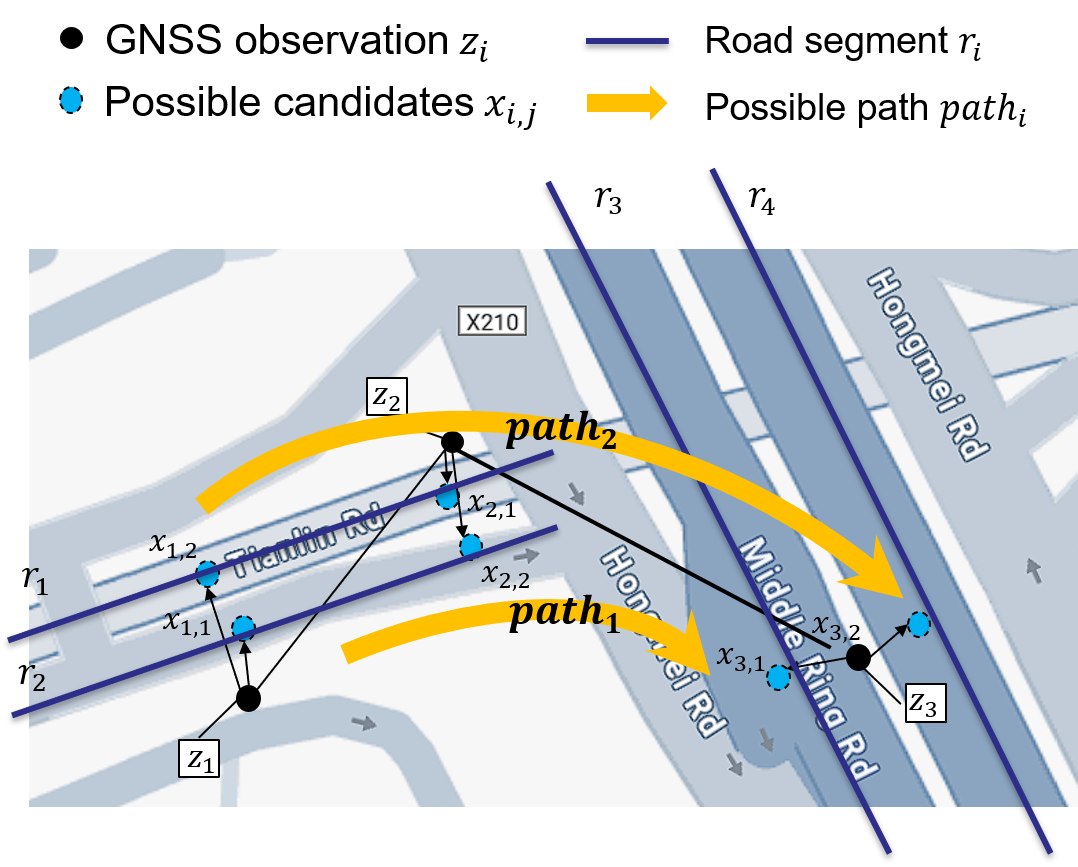
\includegraphics[width=0.8\linewidth]{figs/example.png}
    \caption{Example of map matching problem}
    \label{fig:example}
\end{figure}

\subsection{Posterior Factorization and HMM Components}
Under the Markov assumption, the posterior in \eqref{eq:HMM_MAP} factorizes as
\begin{equation}
    P(X \mid Z) \propto
    \underbrace{\prod_{i=1}^n P(z_i \mid x_i)}_{\text{Emission}}
    \cdot
    \underbrace{\prod_{i=2}^n P(x_i \mid x_{i-1})}_{\text{Transition}}
    \cdot
    P(x_1),
    \label{eq:posterior_factorized}
\end{equation}
where:
\begin{itemize}
    \item $P(z_i \mid x_i)$ is the \emph{emission probability} describing how
          likely a GNSS fix is produced from candidate state $x_i$.
    \item $P(x_i \mid x_{i-1})$ is the \emph{transition probability} describing
          the feasibility of moving between researchen road states.
    \item $P(x_1)$ is the prior distribution for the initial state.
\end{itemize}

The optimal path is computed efficiently via the Viterbi algorithm. Thus,
traditional HMM map matching consists of two foundational components:
\textbf{emission modeling} and
\textbf{transition modeling}.

\subsection{Classical Hidden Markov Model based Map Matching}
\subsubsection{Classical Emission Probability}
In most existing HMM-based map-matching systems (e.g., FMM and many
OpenStreetMap toolchains), the emission probability is modeled as a
fixed, isotropic Gaussian:
\begin{equation}
    P(z_i \mid x_i)
    =
    \frac{1}{2\pi \sigma^2}
    \exp\!\left(
        -\frac{\|z_i - x_i\|^2}{2\sigma^2}
    \right),
    \label{eq:classic_emission}
\end{equation}
where $\sigma$ is an empirically tuned GNSS error standard deviation that
is kept constant over time and space. This choice is attractive because
it is simple, computationally efficient, and easy to calibrate.
However, it assumes that GNSS errors are
(i) stationary in time,
(ii) isotropic in the horizontal plane, and
(iii) independent of the surrounding environment.
As a consequence, it does not exploit the rich uncertainty information
(such as covariance matrices or protection levels) that modern GNSS
receivers can provide.

\subsubsection{Classical Transition Probability}
In the classical formulation, transitions between successive candidate
states are typically modeled through a distance-consistency prior:
\begin{equation}
    P(x_i \mid x_{i-1})
    \propto
    \exp\!\left(
        -\frac{\left|
        d_{\text{road}}(x_{i-1}, x_i)
        -
        d_{\text{gnss}}(z_{i-1}, z_i)
        \right|}{\beta}
    \right),
    \label{eq:classic_transition}
\end{equation}
where $d_{\text{road}}$ is the shortest-path distance on the road graph,
$d_{\text{gnss}}$ is the GNSS-derived displacement between observations
$z_{i-1}$ and $z_i$, and $\beta$ is a smoothing parameter which makes the sum of the probability equals to $1$. This model
favors road paths whose length is consistent with the observed GNSS
motion, while rejecting topologically infeasible transitions (e.g.,
driving against one-way restrictions or crossing disconnected links).

\subsubsection{Dynamic Programming via the Viterbi Algorithm}
Given the factorization in~\eqref{eq:posterior_factorized}, the optimal
state sequence is obtained using the Viterbi algorithm. By propagating
accumulated log-likelihoods forward in time and performing a single
backtracking pass, the algorithm reduces the combinatorial search
from $O(|\mathcal{C}|^n)$ to $O(n \cdot |\mathcal{C}|^2)$, which makes
real-time operation possible on large-scale road networks.
\begin{figure}
    \centering
    \includegraphics[width=1.0\linewidth]{figs/traditionHMM.png}
    \caption{The process of traditional HMM}
    \label{fig:enter-label}
\end{figure}

The above emission and transition models, together with the Viterbi
recursion, constitute the classical HMM-based map-matching framework.
In the following subsection, limitations are discussed with respect
to GNSS stochastic modeling and integrity requirements, which motivates
the GNSS-consistent formulation developed in Section~\ref{sec:proposed}.

% \subsection{Classical Emission and Transition Models}
% % Classical emission with fixed σ^2 I
% % Classical transition model (distance consistency)
% % Short description of Viterbi recursion
% \subsubsection{Classical Emission Probability}
% Most existing systems (e.g., FMM and OpenStreetMap toolchains) adopt a simple
% isotropic Gaussian model:
% \begin{equation}
%     P(z_i \mid x_i)
%     = \frac{1}{2\pi \sigma^2}
%       \exp\!\left( -\frac{\|z_i - x_i\|^2}{2\sigma^2} \right),
%     \label{eq:classic_emission}
% \end{equation}
% where $\sigma$ is a fixed, empirically tuned GNSS error standard deviation.
% Although computationally convenient, this approximation ignores:
% \begin{itemize}
%     \item dynamic variations in GNSS accuracy,
%     \item anisotropy of GNSS error ellipses,
%     \item environment-dependent correlation structures.
% \end{itemize}
% This limitation is the key motivation for the covariance-aware emission model
% developed in this work.

% \subsubsection{Classical Transition Probability}
% Transitions between researchen candidate states are typically modeled as:
% \begin{equation}
%     P(x_i \mid x_{i-1})
%     \propto \exp\!\left(
%         -\frac{\left|
%         d_{\text{road}}(x_{i-1}, x_i)
%         - d_{\text{gnss}}(z_{i-1}, z_i)
%         \right|}{\beta}
%     \right),
%     \label{eq:classic_transition}
% \end{equation}
% where $d_{\text{road}}$ is the shortest-path distance on the road graph,
% $d_{\text{gnss}}$ is the GNSS displacement, and $\beta$ is a smoothing
% parameter. This form encodes a preference for road paths consistent with GNSS
% motion while eliminating topologically invalid transitions (e.g., reverse
% direction on one-way segments).

% \subsubsection{Dynamic Programming via the Viterbi Algorithm}
% Given \eqref{eq:posterior_factorized}, the optimal trajectory is obtained by
% forward propagation of accumulated log-likelihoods and backtracking from the
% final epoch. The Viterbi algorithm reduces computational complexity from
% $O(|\mathcal{C}|^n)$ to $O(n \cdot |\mathcal{C}|^2)$, enabling real-time
% operation in large road networks.
% The above formulation summarizes the classical HMM map-matching method. The
% next section introduces the limitations of this classical model and develops
% a covariance-driven trustworthiness framework that provides more realistic
% probabilities and principled confidence evaluation.

\subsection{Limitations w.r.t.\ GNSS Uncertainty and Integrity}\label{subsec:limitations}
% Explain:
%  - Fixed search radius (not uncertainty-driven)
%  - Euclidean projection (assumes isotropy)
%  - Isotropic emission (σ^2 I) ignores covariance / PL
%  - No trustworthiness / integrity metric
% Reference Fig. 2 comparing classical vs proposed pipeline.


Although classical HMM-based map matching has proven effective in many
applications, its standard formulation exhibits several fundamental
limitations when viewed from the perspective of GNSS stochastic modeling
and integrity requirements. These limitations motivate the development of
the covariance-consistent, integrity-aware framework proposed in the next
section.

\paragraph{Fixed or heuristic candidate search radius.}
Most existing systems use either a constant buffer radius (e.g., 50--300\,m)
or heuristic iterative expansion to retrieve candidate road segments.
Such practices are disconnected from the actual GNSS positioning uncertainty:
the search radius does not enlarge under degraded satellite geometry or reduce
under high-precision conditions. As a result, the candidate set may
under-cover the true road segment in urban canyons or over-cover the network
in open-sky conditions, leading to unnecessary ambiguity and computational
overhead.

\paragraph{Euclidean projection assumes isotropic uncertainty.}
Candidate points are typically generated by orthogonally projecting the GNSS
fix onto nearby road polylines. This implicitly assumes that the GNSS error
distribution is spherical and direction-independent. In reality, GNSS error
ellipses are highly anisotropic and rotate with satellite geometry, multipath,
and blockage. Euclidean projection therefore selects the geometrically closest
point rather than the statistically most plausible one, causing systematic
degradation in challenging environments.

\paragraph{Isotropic emission probability ignores covariance and protection levels.}
Classical emission models adopt a fixed Gaussian likelihood
$\mathcal{N}(0,\sigma^2 I)$, which disregards both
(i) the time-varying covariance matrix provided by modern receivers and  
(ii) the integrity information encoded in protection levels (PLs).
This prevents the HMM from adapting to changes in GNSS quality and fails to
capture the true stochastic structure of the measurement process.

\paragraph{Absence of a principled trustworthiness or integrity indicator.}
The classical HMM returns only the most probable path but does not quantify
how reliable this solution is. In dense urban road networks, multiple
topologically valid paths may be consistent with the GNSS observations, and
the classical framework provides no mechanism to assess ambiguity or detect
potential mismatch events. This limitation is critical for safety-related
applications---such as road pricing, autonomous driving, or integrity
monitoring---where reliability must be quantified, not assumed.

\begin{figure*}[htbp]
    \centering
    % 不再额外缩放，已经是两栏宽度
    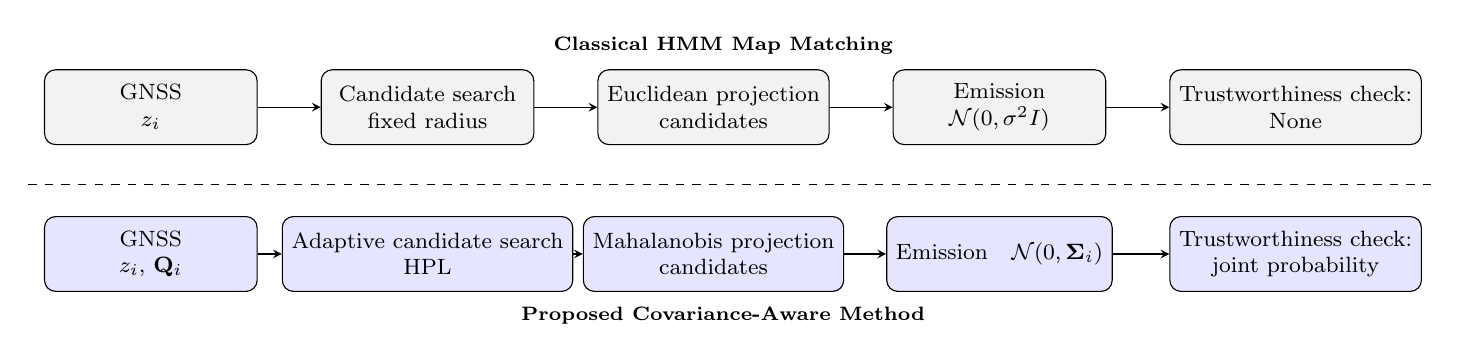
\begin{tikzpicture}[
        >=stealth,
        node distance=0.9cm and 0.8cm,
        box/.style={draw, rounded corners, fill=gray!10,
                    align=center, minimum width=2.7cm,
                    minimum height=0.95cm, font=\footnotesize},
        boxP/.style={draw, rounded corners, fill=blue!10,
                    align=center, minimum width=2.7cm,
                    minimum height=0.95cm, font=\footnotesize}
    ]

    % ------- Classical HMM (top row) -------
    \node[box] (c1) {GNSS \\ $z_i$};
    \node[box, right=of c1] (c2) {Candidate search \\ fixed radius};
    \node[box, right=of c2] (c3) {Euclidean projection \\ candidates};
    \node[box, right=of c3] (c4) {Emission \\ $\mathcal{N}(0,\sigma^2 I)$};
    \node[box, right=of c4] (c5) {Trustworthiness check: \\ None};

    % 行标题：取 c1 和 c4 的中点作为参考点
    \coordinate (ctop) at ($(c1)!0.5!(c5)$);
    \node[above=0.55cm of ctop, font=\scriptsize\bfseries]
        {Classical HMM Map Matching};

    \draw[->] (c1) -- (c2);
    \draw[->] (c2) -- (c3);
    \draw[->] (c3) -- (c4);
    \draw[->] (c4) -- (c5);

    % ------- Proposed (bottom row) -------
    % 注意：逐个 below=of c1,c2,c3,c4，保证四列对齐
    \node[boxP, below=0.9cm of c1] (p1) {GNSS \\ $z_i$, $\mathbf{Q}_i$};
    \node[boxP, below=0.9cm of c2] (p2) {Adaptive candidate search \\  HPL};
    \node[boxP, below=0.9cm of c3] (p3) {Mahalanobis projection \\ candidates};
    \node[boxP, below=0.9cm of c4] (p4) {Emission \
    \ $\mathcal{N}(0,\mathbf{\Sigma}_i)$};
    \node[boxP, below=0.9cm of c5] (p5) {Trustworthiness check: \\ joint probability};

    \coordinate (cbottom) at ($(p1)!0.5!(p5)$);
    \node[below=0.55cm of cbottom, font=\scriptsize\bfseries]
        {Proposed Covariance-Aware Method};

    \draw[->] (p1) -- (p2);
    \draw[->] (p2) -- (p3);
    \draw[->] (p3) -- (p4);
    \draw[->] (p4) -- (p5);

    % dashed separator（画在两行中间）
    \draw[dashed] ($(c1.south west)+(-0.2,-0.5)$) -- ($(c5.south east)+(0.2,-0.5)$);

    \end{tikzpicture}

    \caption{Comparison between classical HMM map matching (top) and the proposed covariance-aware framework (bottom). The proposed method incorporates GNSS covariance, adaptive candidate search, and a Mahalanobis-based emission model.}
    \label{fig:HMM_vs_proposed}
\end{figure*}

\medskip
Figure~\ref{fig:HMM_vs_proposed} summarizes these limitations visually by
contrasting the classical pipeline with the proposed GNSS-consistent,
covariance-aware formulation. The latter addresses all four shortcomings by
replacing heuristic components with probabilistically grounded counterparts.

% ---------------------------------------------------------------------------

\section{GNSS-Consistent HMM and Trustworthiness Evaluation}
\label{sec:proposed}
This section presents an enhanced Hidden Markov Model (HMM)–based map-matching formulation called \textbf{Covariance-aware Map Matching using HMM } that incorporates GNSS positioning uncertainty at three levels: candidate search region definition, candidate point generation, and emission probability modeling. A final subsection introduces a trustworthiness statistic derived from the joint likelihood of the optimal HMM path, enabling consistency evaluation between GNSS observations and the road network. For brevity, the proposed method is referred to as \textbf{CMM-HMM} in the remainder of this paper.

\subsection{GNSS Stochastic Error model and Protection Level}

\subsubsection{GNSS positioning and state covariance}
% WLS formulation, state covariance Σ_z, horizontal covariance Σ_i

The most common positioning method is single-point positioning (SPP). The GNSS position solution and its associated
uncertainty are obtained through a weighted least-squares (WLS) estimation
based on pseudorange observations. 
%========================================================
% WLS covariance derivation for GNSS pseudorange positioning
%========================================================

\subsubsection{Weighted least-squares solution and covariance of GNSS positioning}

\paragraph{Observation model.}
Assume $m$ satellites are tracked at an epoch. The pseudorange observation vector is
\begin{equation}
\boldsymbol{\rho}
=
\begin{bmatrix}
\rho_1 & \rho_2 & \cdots & \rho_m
\end{bmatrix}^{\mathrm{T}},
\end{equation}
and the unknown state is
\begin{equation}
\mathbf{x}
=
\begin{bmatrix}
x & y & z & \delta t
\end{bmatrix}^{\mathrm{T}},
\end{equation}
where $(x,y,z)$ is the receiver position in ECEF and $\delta t$ denotes the receiver clock bias in meters.

For satellite $i$, the linearized pseudo range model can be written as
\begin{equation}
\rho_i
=
r_i(\mathbf{x}) + \delta t + \varepsilon_i,
\end{equation}
where $r_i(\mathbf{x})$ is the geometric range and $\varepsilon_i$ is the measurement noise.

Stacking all measurements yields
\begin{equation}
\boldsymbol{\rho}
=
\mathbf{h}(\mathbf{x}) + \boldsymbol{\varepsilon},
\qquad
\mathbb{E}[\boldsymbol{\varepsilon}]=\mathbf{0},
\qquad
\operatorname{cov}(\boldsymbol{\varepsilon})=\boldsymbol{\Sigma}_{\rho}.
\label{eq:rho_model}
\end{equation}

\paragraph{Linearization.}
Let $\mathbf{x}_0$ be the linearization point and define the increment $\Delta\mathbf{x}=\mathbf{x}-\mathbf{x}_0$.
Using first-order Taylor expansion,
\begin{equation}
\mathbf{h}(\mathbf{x})
\approx
\mathbf{h}(\mathbf{x}_0) + \mathbf{H}\,\Delta\mathbf{x},
\end{equation}
where the Jacobian (geometry) matrix is
\begin{equation}
\mathbf{H}
=
\left.\frac{\partial \mathbf{h}(\mathbf{x})}{\partial \mathbf{x}}\right|_{\mathbf{x}=\mathbf{x}_0}
\in\mathbb{R}^{m\times 4}.
\end{equation}

Define the pre-fit residual (innovation) vector
\begin{equation}
\mathbf{y}
=
\boldsymbol{\rho}-\mathbf{h}(\mathbf{x}_0).
\end{equation}
Then the linearized model becomes
\begin{equation}
\mathbf{y}
=
\mathbf{H}\,\Delta\mathbf{x} + \boldsymbol{\varepsilon}.
\label{eq:lin_model}
\end{equation}

\paragraph{Weighted least-squares estimator.}
Given the weight matrix $\mathbf{W}=\boldsymbol{\Sigma}_{\rho}^{-1}$, the WLS estimate is obtained by minimizing
\begin{equation}
J(\Delta\mathbf{x})
=
(\mathbf{y}-\mathbf{H}\Delta\mathbf{x})^{\mathrm{T}}
\mathbf{W}
(\mathbf{y}-\mathbf{H}\Delta\mathbf{x}).
\end{equation}
Setting $\partial J/\partial \Delta\mathbf{x}=\mathbf{0}$ yields the normal equation
\begin{equation}
\mathbf{H}^{\mathrm{T}}\mathbf{W}\mathbf{H}\,\widehat{\Delta\mathbf{x}}
=
\mathbf{H}^{\mathrm{T}}\mathbf{W}\mathbf{y},
\end{equation}
and therefore
\begin{equation}
\widehat{\Delta\mathbf{x}}
=
(\mathbf{H}^{\mathrm{T}}\mathbf{W}\mathbf{H})^{-1}
\mathbf{H}^{\mathrm{T}}\mathbf{W}\mathbf{y}.
\label{eq:wls_dx}
\end{equation}

\paragraph{Estimation error covariance.}
From \eqref{eq:lin_model} and \eqref{eq:wls_dx}, the estimation error is
\begin{equation}
\widetilde{\Delta\mathbf{x}}
=
\widehat{\Delta\mathbf{x}}-\Delta\mathbf{x}
=
(\mathbf{H}^{\mathrm{T}}\mathbf{W}\mathbf{H})^{-1}
\mathbf{H}^{\mathrm{T}}\mathbf{W}\boldsymbol{\varepsilon}.
\end{equation}
Thus, using $\operatorname{cov}(\boldsymbol{\varepsilon})=\boldsymbol{\Sigma}_{\rho}$ and $\mathbf{W}=\boldsymbol{\Sigma}_{\rho}^{-1}$,

\begin{equation}
\begin{aligned} 
\boldsymbol{\Sigma}_{x}
&=
\operatorname{cov}(\widetilde{\Delta\mathbf{x}})\\
&=
(\mathbf{H}^{\mathrm{T}}\mathbf{W}\mathbf{H})^{-1}
\mathbf{H}^{\mathrm{T}}\mathbf{W}\,
\boldsymbol{\Sigma}_{\rho}\,
\mathbf{W}\mathbf{H}
(\mathbf{H}^{\mathrm{T}}\mathbf{W}\mathbf{H})^{-1}\\
&=
(\mathbf{H}^{\mathrm{T}}\boldsymbol{\Sigma}_{\rho}^{-1}\mathbf{H})^{-1}.
\end{aligned}
\label{eq:wls_cov_full}
\end{equation}

\paragraph{4D and 3D covariance forms.}
If the estimated state is $\mathbf{x}=[x,y,z,\delta t]^{\mathrm{T}}$, then
\begin{equation}
\boldsymbol{\Sigma}_{x}
=
\begin{bmatrix}
\boldsymbol{\Sigma}_{\text{pos}} & \boldsymbol{\Sigma}_{\text{pos},t}\\
\boldsymbol{\Sigma}_{t,\text{pos}} & \sigma_t^2
\end{bmatrix},
\end{equation}
where the $3\times 3$ position covariance is the upper-left block:
\begin{equation}
\boldsymbol{\Sigma}_{\text{pos}}
=
\begin{bmatrix}
\sigma_x^2 & \sigma_{xy} & \sigma_{xz}\\
\sigma_{xy} & \sigma_y^2 & \sigma_{yz}\\
\sigma_{xz} & \sigma_{yz} & \sigma_z^2
\end{bmatrix}.
\label{eq:pos_cov_block}
\end{equation}

% Optional: if you want the 3D covariance after eliminating clock bias via Schur complement:
% \paragraph{(Optional) Position covariance after eliminating clock bias.}
% Partition $\mathbf{H}=[\mathbf{G}\ \ \mathbf{1}]$, where $\mathbf{G}\in\mathbb{R}^{m\times 3}$ is the line-of-sight geometry part
% and $\mathbf{1}\in\mathbb{R}^{m\times 1}$ corresponds to the clock bias column.
% Then the position-only covariance (clock eliminated) can be written using the Schur complement as
% \begin{equation}
% \boldsymbol{\Sigma}_{\text{pos}}
% =
% \left(
% \mathbf{G}^{\mathrm{T}}\mathbf{W}\mathbf{G}
% -
% \mathbf{G}^{\mathrm{T}}\mathbf{W}\mathbf{1}\,
% (\mathbf{1}^{\mathrm{T}}\mathbf{W}\mathbf{1})^{-1}
% \mathbf{1}^{\mathrm{T}}\mathbf{W}\mathbf{G}
% \right)^{-1}.
% \label{eq:schur_pos_cov}
% \end{equation}

% Let $\boldsymbol{\rho} \in \mathbb{R}^{m}$
% denote the vector of pseudorange measurements from $m$ visible satellites.
% The linearized pseudorange observation model at epoch $i$ can be written as
% \begin{equation}
% \boldsymbol{\rho}
% =
% \mathbf{H}\,\boldsymbol{z}
% +
% \boldsymbol{\varepsilon},
% \label{eq:pseudo_range_linear}
% \end{equation}
% where $\boldsymbol{z} = [x\; y\; z\; c\Delta t]^{\mathrm{T}}$ is the user
% position and receiver clock bias state vector,
% $\mathbf{H} \in \mathbb{R}^{m \times 4}$ is the geometry (design) matrix composed
% of line-of-sight unit vectors, and $\boldsymbol{\varepsilon}$ denotes the
% pseudorange measurement noise.
% \begin{equation}
% \mathbf{H}
% =
% \begin{bmatrix}
% -\ell_{x,1} & -\ell_{y,1} & -\ell_{z,1} & 1 \\
% -\ell_{x,2} & -\ell_{y,2} & -\ell_{z,2} & 1 \\
% \vdots      & \vdots      & \vdots      & \vdots \\
% -\ell_{x,m} & -\ell_{y,m} & -\ell_{z,m} & 1
% \end{bmatrix},
% \label{eq:H_matrix}
% \end{equation}
% where $(\ell_{x,k}, \ell_{y,k}, \ell_{z,k})$ denote the components of the 
% line-of-sight (LOS) unit vector from the user to satellite $k$, 
% and the last column of $\mathbf{H}$ equals $1$ because the pseudorange 
% measurement is only dependent on the receiver clock bias.


% Assuming zero-mean pseudorange residuals with covariance
% $\boldsymbol{\Sigma}_{\rho}$, the WLS solution in iterative form is given by
% \begin{equation}
% \hat{\boldsymbol{z}}
% =
% \left( \mathbf{H}^{\mathrm{T}}
% \boldsymbol{\Sigma}_{\rho}^{-1}
% \mathbf{H} \right)^{-1}
% \mathbf{H}^{\mathrm{T}}
% \boldsymbol{\Sigma}_{\rho}^{-1}
% \boldsymbol{\rho}.
% \label{eq:wls_solution}
% \end{equation}
% The corresponding estimation error covariance of the navigation state is

% \begin{equation}   
%     \boldsymbol{\Sigma}_{i}
%     =
%     \left(
%     \mathbf{H}^{\mathrm{T}}
%     \boldsymbol{\Sigma}_{\rho}^{-1}
%     \mathbf{H}
%     \right)^{-1}\\
%     =
%     \begin{bmatrix}
%     \sigma_x^2 & \sigma_{xy} & \sigma_{xz}\\
%     \sigma_{xy} & \sigma_y^2 & \sigma_{yz}\\
%     \sigma_{xz} & \sigma_{yz} & \sigma_z^2
%     \end{bmatrix}
%     \label{eq:state_cov}
% \end{equation}

% % The horizontal positioning covariance used in map matching is obtained by
% % extracting the position-related submatrix:
% % \begin{equation}
% % \boldsymbol{\Sigma}_i
% % =
% % \begin{bmatrix}
% % \sigma_x^2 & \sigma_{xy} & \sigma_{xz}\\
% % \sigma_{xy} & \sigma_y^2 & \sigma_{yz}\\
% % \sigma_{xz} & \sigma_{yz} & \sigma_z^2
% % \end{bmatrix},
% % \label{eq:horizontal_cov}
% % \end{equation}
% where $\sigma_x^2$ and $\sigma_y^2$ denote the variances in the east and north
% directions, respectively. The illustration of GNSS covariance is shown in \ref{fig:covariance}

\begin{figure}[htbp]
    \centering
    \includegraphics[width=1\linewidth]{figs/covariance.png}
    \caption{Visual representation of the GNSS positioning covariance calculation process. The final position uncertainty (Right) is a function of the satellite geometry matrix $\mathbf{H}$ (Left) and the pseudorange measurement noise $\boldsymbol{\Sigma}_{\rho}$ (Middle). This process results in the anisotropic error ellipse $\boldsymbol{\Sigma}_i$ used in our probability emission model.}
    \label{fig:covariance}
\end{figure}

In practical GNSS receivers, this covariance matrix is often made available
through standard output messages such as the NMEA \texttt{GST} sentence, which
provides axis-aligned or rotated confidence ellipse parameters that can be
converted into $\boldsymbol{\Sigma}_{pos}$. This covariance encapsulates the
combined effects of satellite geometry, atmospheric errors, multipath, and
measurement noise, and therefore serves as the statistical basis for the
covariance-aware emission probability model introduced in the following
subsection.

\subsubsection{Integrity monitoring and horizontal protection level}
% RAIM/ARAIM description, PL / HPL_i, final r_i = HPL_i
Protection Level (PL) is a widely adopted integrity metric that provides a conservative upper bound on the horizontal position error for a specified integrity risk level (e.g., $10^{-5}$ or $10^{-7}$). The protection level (PL) denotes the threshold below which the true horizontal position error lies with integrity risk not exceeding $10^{-5}$, that is,
\begin{equation}
\Pr\!\left( |e_{\mathrm{hor}}| > \mathrm{PL} \right) \le 10^{-5}.
\label{eq:protection level}
\end{equation}

In integrity monitoring, the PL is an alternative representation of the integrity risk bound. Rather than directly computing the probability of hazardous misleading information (HMI), the PL expresses the maximum position-domain error that would remain safe under a specified integrity requirement. This makes PL a more practical and receiver-agnostic quantity, especially when the alert limits (ALs) of downstream applications are unknown to the GNSS receiver.

The PL corresponding to the integrity risk expression can be computed iteratively using the nonlinear equation

\begin{equation}
\begin{aligned}
\mathrm{I_{REQ}}
&<
2\, Q\!\left( \frac{\mathrm{PL} - b_0}{\sigma_0} \right)
+
\sum_{i=1}^{h}
Q\!\left(
\frac{\mathrm{PL} - T\Delta_i - b_i}{\sigma_i}
\right) P_{H_i}  \\
&\quad
+\, P_{NM},
\end{aligned}
\label{eq:pl_iterative}
\end{equation}

where $Q(\cdot)$ is the standard Gaussian tail probability, $(b_0, \sigma_0)$ denote the nominal bias and standard deviation, $(b_i, \sigma_i)$ and $P_{H_i}$ are the corresponding parameters under fault mode $i$, $T\Delta_i$ represents the solution-separation term for the $i$-th fault hypothesis, and $P_{NM}$ is the probability of non-monitored fault modes. 

The resulting PL encapsulates the same integrity information as the underlying risk model but in a form readily usable by downstream safety-critical applications. In this work, the Horizontal Protection Level (HPL) obtained from \eqref{eq:pl_iterative} is used as the radius of the candidate search region in covariance-aware map matching.

\begin{figure}[htbp]
    \centering
    \includegraphics[width=1\linewidth]{figs/PL.png}
    \caption{The illustration of protection level}
    \label{fig:PL}
\end{figure}

Two major algorithms exist for computing HPL:

\paragraph{Residual-based HPL (RAIM)}
In classical Receiver Autonomous Integrity Monitoring (RAIM), GNSS measurements are checked for consistency using residual tests. Let $\mathbf{H}$ denote the geometry matrix and $\mathbf{W}$ the weighting matrix. The position-domain covariance is obtained as
\begin{equation}
\boldsymbol{\Sigma}_{\mathrm{pos}}
=
\left( \mathbf{H}^{\mathrm{T}} \mathbf{W} \mathbf{H} \right)^{-1}.
\end{equation}
The horizontal standard deviation is
\begin{equation}
\sigma_{\mathrm{H}}
=
\sqrt{\sigma_x^2 + \sigma_y^2},
\end{equation}
and the protection level is computed as
\begin{equation}
\mathrm{HPL}_{\mathrm{RAIM}}
=
K_{\mathrm{RAIM}} \, \sigma_{\mathrm{H}},
\end{equation}

where $K_{\mathrm{RAIM}}$ depends on the false-alarm and missed-detection probabilities. This method is computationally simple but assumes a single-fault model with Gaussian errors.

\paragraph{MHSS-based HPL (ARAIM).}

Advanced RAIM (ARAIM) adopts the Multiple Hypothesis Solution Separation (MHSS) framework, which explicitly accounts for multiple satellite fault hypotheses. For each fault mode $f \in \mathcal{F}$, a solution-separation vector is computed. The horizontal protection level is then

\begin{equation}
\mathrm{HPL}_{\mathrm{MHSS}}
=
\max_{f \in \mathcal{F}}
\left(
| S_f | 
+
K_f \, \sigma_{\mathrm{H},f}
\right),
\end{equation}
where $S_f$ is the solution-separation bias, $\sigma_{\mathrm{H},f}$ is the protected standard deviation under mode $f$, and $K_f$ is the integrity coefficient for that mode. This method provides statistically rigorous integrity guarantees and incorporates fault geometry explicitly.


\subsection{GNSS-Consistent HMM Map Matching}
\label{subsec:gnss_consistent_hmm}

This section reformulates the HMM map-matching framework so that all core
elements---states, observations, candidate generation, and emission
likelihoods---are explicitly consistent with the stochastic GNSS error model.
Unlike the classical formulation, which assumes fixed isotropic uncertainty,
the proposed framework incorporates the full covariance information
$\boldsymbol{\Sigma}_i$ (or equivalently PL-based bounds) provided by modern GNSS
receivers. This establishes a unified probabilistic treatment of uncertainty
throughout the entire HMM pipeline.

\subsubsection{States and Observations with Covariance}
\label{subsubsec:states_observations}

Let
\[
z_i \in \mathbb{R}^2
\]
denote the horizontal GNSS position estimate at epoch $i$, and let
\[
\boldsymbol{\Sigma}_i \in \mathbb{R}^{2\times 2}
\]
be the corresponding GNSS positioning covariance matrix obtained from the
weighted least-squares (WLS) solution or receiver-reported confidence ellipse
(e.g., NMEA \texttt{GST}). The pair $(z_i, \boldsymbol{\Sigma}_i)$ therefore
represents a stochastic observation whose uncertainty is explicitly modeled.

Given the uncertainty-aware candidate search region (e.g., the
HPL-based disk $\Omega_i$), the set of feasible road segments for epoch $i$
is
\[
\mathcal{C}_{\mathrm{seg},i}
=
\{\, s \in \mathcal{G} : s \cap \Omega_i \neq \varnothing \,\}.
\]

Each state in the HMM corresponds to a specific candidate point obtained by
projecting the GNSS observation onto one of these segments using the
Mahalanobis projection operator:
\[
x_{i,j}
\in
\mathcal{C}_{\mathrm{pnt},i}
=
\Big\{
\arg\min_{x \in s_j}
f(z_i - x)^{\mathrm{T}} \boldsymbol{\Sigma}_i^{-1} (z_i - x)
\;\Big|\;
s_j \in \mathcal{C}_{\mathrm{seg},i}
\Big\}.
\]

Thus, for each epoch $i$, the HMM state set is the uncertainty-consistent
candidate collection
\[
\mathcal{C}_{pnt,i} = \{ x_{i,1}, x_{i,2}, \ldots \},
\]
and the emission probability model and transition model defined in later
subsections operate entirely on this covariance-aware state representation.

By embedding GNSS covariance directly into the observation model and candidate
generation process, the resulting HMM formulation provides a statistically
accurate description of the measurement process and forms the basis for both
improved map-matching accuracy and integrity-aware trustworthiness evaluation.



\subsubsection{HPL-based candidate segment search}
% Your candidate road segment search using Ω_i and HPL_i
Conventional HMM-based map matching methods typically retrieve candidate road segments by applying a fixed-radius buffer around each GNSS observation. Such a static search range does not account for the time-varying nature of GNSS measurement quality, which is strongly influenced by satellite geometry, multipath, and environmental occlusions. In the formulation of Paul \cite{HMM}, for example, a constant search radius of 300 m is employed regardless of the underlying positioning uncertainty. Some subsequent studies introduce heuristic, iteratively expanded search radii to control computational complexity by maintaining the number of retrieved candidate segments within a predefined range. Under sparse road conditions, the search radius is enlarged (e.g., doubled) to ensure a sufficient number of candidate states, whereas in dense urban networks the radius is reduced to avoid an excessive candidate set. Although such adaptive heuristics provide partial mitigation, they remain detached from the physical stochastic properties of GNSS measurements and therefore lack principled statistical grounding.

To address this, we introduce an \textbf{adaptive, integrity-driven search region} based on the horizontal protection level (HPL). Conventional fixed-radius candidate search fails to reflect real-time variations in GNSS positioning uncertainty. In this study, the search region is determined using the \textbf{Horizontal Protection Level (HPL)}. Given the horizontal protection level (HPL) estimated by either RAIM or ARAIM,
the candidate search radius at epoch $i$ is defined as
\begin{equation}
r_i = \mathrm{HPL}_i .
\end{equation}
By definition, the HPL guarantees that the true horizontal position error does
not exceed $r_i$ with the specified integrity risk. Therefore, all road segments
that intersect the corresponding HPL-based search region are considered valid
candidates for map matching at epoch $i$.

Let $z_i \in \mathbb{R}^2$ denote the GNSS position estimate at epoch $i$, and
define the HPL-induced search region as the closed disk
\begin{equation}
\Omega_i
=
\left\{
x \in \mathbb{R}^2 \;\middle|\; \| x - z_i \|_2 \le r_i
\right\},
\end{equation}
where $\| \cdot \|_2$ denotes the Euclidean norm in the horizontal plane.

Let $\mathcal{G}$ denote the road network, represented as a set of road segments
embedded in $\mathbb{R}^2$. The candidate road segment set for epoch $i$ is then
defined as
\begin{equation}
\mathcal{C}_{\text{seg},i}
=
\left\{
s \in \mathcal{G}
\;\middle|\;
s \cap \Omega_i \neq \varnothing
\right\},
\label{eq:candidate_set}
\end{equation}
i.e., all road segments that geometrically intersect the HPL-based search region.

This HPL-driven candidate selection strategy ensures:
\begin{itemize}
    \item expanded search regions under degraded GNSS conditions,
    \item compact and efficient search under open-sky environments,
    \item integrity-consistent and parameter-free candidate generation
          without ad hoc tuning.
\end{itemize}

\begin{figure}[htbp]
    \centering
    \includegraphics[width=1\linewidth]{figs/PLsearch.png}
    \caption{The illustration of road segment candidates search by protection level}
    \label{fig:PL}
\end{figure}


\subsubsection{Mahalanobis-based candidate point projection}
% Your Mahalanobis projection section and figures
Traditional HMM-based map-matching algorithms compute candidate points by performing a Euclidean orthogonal projection of each GNSS observation onto nearby road polylines. This procedure implicitly assumes an \emph{isotropic} GNSS error model, meaning that the uncertainty is the same in all directions. However, real GNSS positioning errors are highly \emph{anisotropic}, producing elongated covariance ellipses whose principal axes vary with satellite geometry and multipath.

To account for this anisotropy, we adopt the \textbf{Mahalanobis projection} operator, which projects GNSS observations onto road segments in a manner consistent with the covariance structure. The Mahalanobis projection admits an equivalent geometric interpretation that further clarifies its advantage over Euclidean projection. Let $\boldsymbol{\Sigma}_i = \mathbf{L}_i \mathbf{L}_i^{\mathrm{T}}$ be the Cholesky factorization of the GNSS covariance matrix. By applying the linear whitening transformation

\begin{equation}
\tilde{z}_i = \mathbf{L}_i^{-1} z_i, 
\quad
\tilde{x} = \mathbf{L}_i^{-1} x
\end{equation}

the anisotropic covariance ellipse in the original coordinate frame is mapped to an isotropic unit circle in the whitened space. Under this transformation, the Mahalanobis distance satisfies

\begin{equation}
    \left(z_i - x\right)^{\mathrm{T}} \boldsymbol{\Sigma}_i^{-1} \left(z_i - x\right)
=
\|\tilde{z}_i - \tilde{x}\|_2^{\,2}
\end{equation}

which means that Mahalanobis projection in the original coordinates is exactly equivalent to Euclidean orthogonal projection in the whitened coordinates. Thus, the proposed approach can be interpreted as performing projection after shaping the coordinate frame so that the GNSS uncertainty becomes spherical. 

\begin{figure}[htbp]
    \centering
    \includegraphics[width=1\linewidth]{figs/maha_vs_eu.png}
    \caption{Illustration of Euclidean projection versus Mahalanobis projection under an anisotropic GNSS covariance ellipse. }
    \label{fig:measprob}
\end{figure}

This perspective highlights that the Mahalanobis projection is the statistically appropriate projection operator when GNSS errors are anisotropic, whereas Euclidean projection implicitly assumes a spherical uncertainty model that is generally violated in practical GNSS environments. Intuitively, the covariance matrix defines a family of nested error ellipses representing iso-likelihood contours of the GNSS positioning error: inner ellipses correspond to higher posterior probability and outer ellipses to lower probability. Under the Mahalanobis metric, projecting a GNSS observation onto a road segment is equivalent to identifying the point on that segment that lies on the smallest error ellipse intersecting the road. This point is, in turn, the candidate location with the highest likelihood of being the true position under the anisotropic error model. In contrast to Euclidean projection—which selects the geometrically nearest point without regard to the underlying uncertainty geometry—the Mahalanobis projection selects the statistically most plausible candidate consistent with the full covariance structure, as shown in \ref{fig:measprob}.

The candidates are generated as following steps. For the $i\ th$ GNSS observation $z_i$ and corresponding candidate road segment $s_j$ in the segment candidates set , the projected point is defined as
\begin{equation}
x_{i,j}
=
\arg\min_{x \in s_j}
\left( z_i - x \right)^{\mathrm{T}}
\boldsymbol{\Sigma}_i^{-1}
\left( z_i - x \right),
\label{eq:ma_project}
\end{equation}
where $\boldsymbol{\Sigma}_i$ is the $2\times 2$ horizontal covariance matrix reported by the GNSS receiver.

The resulting set of candidate points is
\begin{equation}
\mathcal{C}_{pnt,i}
=
\left\{
x_{i,j}
\;\middle|\;
j:r_j \in \mathcal{C}_{seg,i}
\right\},
\end{equation}
where $\mathcal{C}_{seg,i}$ denotes the set of candidate segments obtained from the HPL-based search region. This covariance-consistent projection provides several advantages:
\begin{itemize}
    \item it aligns the projection direction with the principal axes of the GNSS error ellipse;
    \item it avoids selecting candidates that lie along high-uncertainty axes, even if they are geometrically closer;
    \item it naturally adapts to time-varying and environment-dependent GNSS uncertainty statistics.
\end{itemize}

\begin{figure}[htbp]
    \centering
    \includegraphics[width=1\linewidth]{figs/measprob.png}
    \caption{Illustration of Euclidean projection versus Mahalanobis projection under an anisotropic GNSS covariance ellipse. 
    The red point denotes the GNSS observation $z_i$; 
    the yellow point is the Euclidean (orthogonal) projection onto the road segment; 
    the green point is the Mahalanobis projection that minimizes the covariance-weighted distance. 
    Because the GNSS error ellipse is elongated, the Mahalanobis projection correctly selects the candidate aligned with the principal axis of uncertainty, whereas the Euclidean projection incorrectly favors the geometrically closest point.}
    \label{fig:measprob}
\end{figure}


\subsubsection{Covariance-based Gaussian emission probability}
% Your emission probability with Σ_i and discussion (shorter; refer back to 3.1 for Σ_i)
Given an observation $z_i$ and a candidate state $x_{i,j}$, the emission
probability is modeled using a bivariate Gaussian distribution governed by the
GNSS covariance matrix:
\begin{equation}
p(z_i \mid x_{i,j})
=
\frac{1}{2\pi \sqrt{|\boldsymbol{\Sigma}_i|}}
\exp\!\left[
-\frac{1}{2}
\mathbf{d}_{i,j}^{\mathrm{T}}
\boldsymbol{\Sigma}_i^{-1}
\mathbf{d}_{i,j}
\right],
\label{eq:cov_emission}
\end{equation}
where the positioning residual is
\[
\mathbf{d}_{i,j} = z_i - x_{i,j}.
\]

Compared with the classical fixed-variance isotropic likelihood
$\mathcal{N}(0,\sigma^2I)$, the covariance-based model incorporates the
full GNSS error geometry and therefore

\begin{itemize}
    \item adapts automatically to real-time GNSS quality,
    \item tightens the likelihood when satellite geometry is good, 
    \item avoids overconfidence in degraded environments,
    \item remains statistically consistent with the underlying GNSS stochastic model.
\end{itemize}

\subsection{Normalized Joint Likelihood and Trustworthiness Statistic}

\subsubsection{Normalization of emission and transition probabilities}
% Eq. for \tilde{p}(z_i | x_{i,j}), normalization across j
% Transition normalization π_i(j,k), conservation of probability mass
At each epoch $i$, the emission probabilities computed for different candidate
states $\{x_{i,j}\}$ may vary significantly in magnitude due to changes in GNSS
covariance, Mahalanobis distance scale, and road density. To remove this scale
dependency, the emission probabilities are normalized across all candidates
within the same epoch:
\begin{equation}
\tilde{p}(z_i \mid x_{i,j})
=
\frac{
p(z_i \mid x_{i,j})
}{
\sum\limits_{k} p(z_i \mid x_{i,k}) + \varepsilon
},
\label{eq:normalized_emission}
\end{equation}
where $\varepsilon$ is a small numerical constant preventing division by zero.
This normalization ensures that
\begin{equation}
\sum_{j} \tilde{p}(z_i \mid x_{i,j}) = 1,
\end{equation}
allowing the emission probabilities to be interpreted as a discrete probability
distribution over all candidate states at epoch $i$.

\subsubsection{Normalization of Emission and Joint Probabilities}

Similarly, when combined with transition probabilities, the joint probability
mass of all feasible state transitions between consecutive epochs is conserved.
That is, for each epoch, the sum of probabilities over all admissible transfer
routes, defined by the product of normalized emission probabilities and
topology-consistent transition probabilities, is equal to one. 

For each epoch $i$, define the (unnormalized) transition weights
\begin{equation}
w_i(j,k)
=
\tilde{p}(z_i \mid x_{i,k}) \,
p(x_{i,k} \mid x_{i-1,j}),
\end{equation}
and the corresponding normalized transition probabilities
\begin{equation}
\begin{aligned}
\pi_i(j,k)
&=
\frac{
    w_i(j,k)
}{
    \displaystyle
    \sum_{j'} \sum_{k'}
    w_i(j',k')
}\\
&=
\frac{
    \tilde{p}(z_i \mid x_{i,k}) \,
    p(x_{i,k} \mid x_{i-1,j})
}{
    \displaystyle
    \sum_{j'} \sum_{k'}
    \tilde{p}(z_i \mid x_{i,k'}) \,
    p(x_{i,k'} \mid x_{i-1,j'})
}.
\end{aligned}
\label{eq:transition_norm}
\end{equation}
By construction, the total probability mass over all admissible transfer routes
between epochs $i-1$ and $i$ is conserved:
\begin{equation}
\sum_{j} \sum_{k} \pi_i(j,k) = 1.
\end{equation}

Finally, the optimal matched trajectory $X^\star$ is obtained using the Viterbi
algorithm:
\begin{equation}
X^\star = \arg\max_X p(Z \mid X).
\end{equation}

To deal with spike in certain epoch while preventing decline caused by the probability decentralization, the normalized log-likelihood of the optimal path is defined as a
trustworthiness statistic for a given window-slide length with total $l$ epochs:
\begin{equation}
T
=
\sum_{i=n}^{n+l}
\left[
\log \tilde{p}(z_i \mid x_i^\star)
+
\log p(x_i^\star \mid x_{i-1}^\star)
\right].
\label{eq:trustworthiness}
\end{equation}

As a result, the
HMM recursion redistributes probability mass across competing path hypotheses
without artificial inflation or attenuation caused by numerical scaling.

This normalized formulation provides three key benefits: (i) it removes
sensitivity to covariance determinant magnitude, (ii) it enhances numerical
stability for long trajectories, and (iii) it enables meaningful aggregation of
likelihood information across time.


\subsubsection{Trustworthiness interpretation and definition of $T$}
% Definition of p(Z | X), Viterbi for X*, trust score T (normalized log-likelihood)
% Interpretation: high T vs low T, ambiguity and mismatch, ROC / integrity use
Let $Z=\{z_1,\ldots,z_N\}$ denote a sequence of GNSS observations and
$X=\{x_1,\ldots,x_N\}$ a corresponding state sequence on the road network.
The normalized joint likelihood under the HMM formulation is
\begin{equation}
p(Z \mid X)
=
\prod_{i=1}^{N}
\tilde{p}(z_i \mid x_i)
\,
p(x_i \mid x_{i-1}),
\end{equation}
where $p(x_i \mid x_{i-1})$ enforces road connectivity, legal travel direction,
and shortest-path consistency.

Beyond trajectory estimation, the magnitude of the resulting joint probability
provides a direct measure of consistency between GNSS observations and the road
network structure. In simple road environments or under high-quality GNSS
conditions, this probability mass concentrates on a small number of compatible
paths, yielding a high-confidence solution. In contrast, in complex road
networks—such as dense urban grids or parallel-road scenarios—multiple
topologically plausible transitions coexist, causing the probability mass to be
distributed among competing paths. This dispersion is a fundamental driver of
map-matching ambiguity and mismatch events.

A higher value of $T$ indicates strong mutual consistency between the GNSS
measurements and road connectivity constraints, whereas a lower value signals
increased ambiguity or potential mismatch risk. Since $T$ intrinsically reflects
both measurement uncertainty and road-network complexity, thresholding this
statistic enables quantitative integrity checks, receiver operating
characteristic (ROC) analysis, and systematic evaluation of availability–
integrity trade-offs in safety-critical navigation applications.
It should be noted that the GNSS positioning covariance obtained from WLS estimation reflects uncertainty only under the nominal, fault-free hypothesis. In the presence of unmodeled multipath or satellite faults, the covariance may become over-optimistic and fail to bound the true position error. For this reason, integrity metrics such as protection level are incorporated in candidate selection, avoids missing the truth even when covariance is optimistic and preserves availability. Meanwhile, even when GNSS covariance becomes over-optimistic due to unmodeled multipath or faults, inconsistencies between the covariance-based emission likelihood and road-network-constrained transitions cause the joint HMM likelihood to drop, allowing the proposed trustworthiness statistic to flag unreliable map-matching results without relying on covariance alone.


\subsection{Summary of GNSS-Consistent HMM Formulation and Trustworthiness}

\begin{algorithm}[t]
\caption{CMM-HMM Algorithm.}
\label{alg:cmm_hmm}
\begin{algorithmic}[1] % The [1] enables line numbering
\State Initialize road network $\mathcal{G}$, GNSS trajectory $Z$, covariance sequence $\mathbf{\Sigma}$, HPL sequence $\mathbf{r}$, and UBODT table $\mathcal{U}$.
\State Initialize transition trellis $\mathcal{T}$ and candidate sets $\mathcal{C}_{1 \dots N} \leftarrow \varnothing$.
\For{$i = 1, 2, \dots, N$}
    \State Define adaptive search region $\Omega_i$ using HPL radius $r_i$ (Eq. 11).
    \State Query candidate segments $\mathcal{C}_{\mathrm{seg},i} \leftarrow \{ s \in \mathcal{G} : s \cap \Omega_i \neq \varnothing \}$.
    \If{$\mathcal{C}_{\mathrm{seg},i} = \varnothing$} 
        \State \textbf{return} Failure (Gap in Coverage)
    \EndIf
    \For{\textbf{each} segment $s_j \in \mathcal{C}_{\mathrm{seg},i}$}
        \State Compute Mahalanobis projection $x_{i,j}$ minimizing $\mathbf{d}^T \boldsymbol{\Sigma}_i^{-1} \mathbf{d}$ (Eq. 14).
        \State Calculate covariance-based likelihood $L_{i,j}$ (Eq. 15).
        \State $\mathcal{C}_{\mathrm{pnt},i} \leftarrow \mathcal{C}_{\mathrm{pnt},i} \cup \{x_{i,j}\}$.
    \EndFor
    \State Normalize emission probabilities $\tilde{p}(z_i | x_{i,j})$ using Eq. (16).
\EndFor
\State Initialize Viterbi path variables $\delta_1(j) \leftarrow \tilde{p}(z_1 | x_{1,j})$ for all $j$.
\For{$i = 2, 3, \dots, N$}
    \For{\textbf{each} candidate $x_{i,k} \in \mathcal{C}_{\mathrm{pnt},i}$}
        \State Find optimal parent $x^\star_{i-1}$ maximizing $\delta_{i-1}(j) \cdot p(x_{i,k} | x_{i-1,j})$.
        \State Update path probability $\delta_{i}(k)$ and store backpointer $\psi_{i}(k)$.
    \EndFor
\EndFor
\State Backtrack via $\psi$ to retrieve optimal path $X^\star = \{x_1^\star, \dots, x_N^\star\}$.
\State Compute Trustworthiness $T \leftarrow \frac{1}{N} \sum_{i=1}^{N} \ln \left( \tilde{p}(z_i | x_i^\star) \cdot p(x_i^\star | x_{i-1}^\star) \right)$ (Eq. 22).
\State \textbf{return} $X^\star, T$
\end{algorithmic}
\end{algorithm}


By incorporating integrity-aware candidate search based on protection level
and covariance-aware emission probability modeling, an enhanced HMM-based
map-matching framework is obtained. Under this formulation, the most probable
road-constrained trajectory is determined by maximizing the joint likelihood
between the GNSS observations and the road-network-constrained state sequence.
From a Bayesian perspective, this procedure already yields a statistically
optimal map-matching solution in the maximum \emph{a posteriori} (MAP) sense.

However, for safety-critical applications such as navigation charging,
autonomous driving support, or integrity monitoring, providing only a
single best-matching result is insufficient. In addition to the estimated road
trajectory, the navigation system must also quantify how reliable this result
is. In practice, map-matching failures tend to occur in environments where
GNSS observations are degraded and multiple topologically plausible road
sequences are simultaneously consistent with the measurements. Therefore,
the \emph{trustworthiness} of a map-matching result should explicitly reflect
the degree of consistency between GNSS observations and the underlying road
network constraints.

\begin{figure}
    \centering
    \includegraphics[width=1.0\linewidth]{figs/trustworthiness.png}
    \caption{Trustworthiness in different road segments}
    \label{fig:trustworthiness}
\end{figure}

The joint probability inherent to the HMM formulation naturally encodes this
consistency and thus provides a principled basis for trustworthiness
evaluation. Nevertheless, raw likelihood values are sensitive to scale effects
introduced by covariance magnitude, candidate set size, and trajectory length.
To enable meaningful comparison across epochs and scenarios, additional
normalization and interpretation are required.

\section{Simulation Study}
\label{sec:simulation}
% 一定要带上前面的公式，用公式几生成了什么

This section aims to verify that proposed emission probability and transition probability is accurate in controlled nominal environment, shows priority of CMM to HMM in accuracy as long as availability, and gives illustration on the mechanism of proposed trustworthiness change in different level of road network complexity and observation bias.

Monte-Carlo experiment is carried on the condition of pseudo range standard derivation. By adding a random noise of gaussian model to the distance between synthetic constellation and ground truth, pseudo range is generated and observation of vehicle position can be obtained by weighed least square algorithm. This simulation aims at three aspects:

\begin{enumerate}

    \item \textbf{Probabilistic model validation under nominal condition:}
    By conducting a statistical comparison between the Monte Carlo simulation results and those produced by the proposed model, the validity of the model under the specified assumptions can be assessed, equation \ref{eq:wls_cov_full}, equation \ref{eq:protection level}, equation \ref{eq:classic_transition} namely.

    \item \textbf{Trustworthiness evolution analysis:}
    Statistic analysis on the proposed trustworthiness is conducted to show its sensitivity to sigma, road network complexity and window length.
    % The third objective is to analyze the computational efficiency and robustness
    % of the proposed framework through ablation and sensitivity studies.
    % By selectively enabling or disabling key components—such as covariance-based
    % emission modeling, adaptive candidate search, and Mahalanobis projection—the
    % simulation quantifies their individual and combined contributions.
    % Sensitivity analyses with respect to horizontal bias, covariance scaling, and
    % candidate search parameters are conducted to assess how the proposed method
    % responds to GNSS uncertainty mis-calibration and extreme error conditions,
    % which are commonly encountered in real-world deployments.

    \item \textbf{Accuracy enhancement via adaptive candidate search regions and trustworthiness effectives:} By introducing Mahalanobis-projection in equation \ref{eq:ma_project} and search region from \ref{eq:protection level}, matching results shows less error in CMM compared with HMM. And to evaluate the effectiveness of the proposed trustworthiness metric in discriminating between correct and mismatched map-matching results by ROC curve.
    % avalibility定性说，不要再标题说，
    % efficiency如果要说，要给出可量化可计算的指标
    % 顺序要调整成trustworthiness在第二点，最后介绍整体的效果。
    % The second objective is to investigate how adaptive candidate search regions,
    % defined by the horizontal protection level (HPL) or, when HPL is unavailable,
    % by a covariance-ellipse-based surrogate, affect candidate coverage and
    % matching availability under degraded GNSS conditions.
    % This objective targets scenarios in which classical fixed-radius candidate
    % search may fail to include the true road segment due to large positioning
    % errors or biases.
    % The simulation study examines whether the proposed integrity-consistent
    % candidate selection strategy can recover valid candidates that are otherwise
    % missed, thereby increasing the availability of map-matching outputs while
    % maintaining consistency with GNSS uncertainty information.
    
\end{enumerate}

% This section presents a comprehensive simulation study designed to validate the
% proposed GNSS-covariance-consistent HMM map-matching framework under controlled
% and reproducible conditions.
% While real-vehicle experiments are essential for demonstrating practical
% feasibility, simulation enables systematic control of GNSS error statistics,
% road-network complexity, and failure modes, which is critical for isolating the
% effects of uncertainty modeling and integrity-aware candidate selection.

% The simulation framework is constructed to mirror the probabilistic assumptions
% introduced in Section~III, including covariance-aware emission modeling,
% adaptive candidate search based on protection level or covariance ellipse, and
% the proposed trustworthiness statistic.
% By generating ground-truth trajectories on a known road network and injecting
% GNSS errors with prescribed covariance and bias characteristics, the simulation
% study allows direct comparison between the proposed method and a classical
% HMM-based baseline with fixed isotropic error assumptions.
% In addition to accuracy evaluation, particular emphasis is placed on availability,
% candidate coverage, and robustness, which are key performance indicators for
% safety-critical map-matching applications.

% \subsection{Objectives of the Simulation Study}
% \label{sec:sim_objective}



\subsection{Simulation Environment and Ground-Truth Generation}
\label{sec:sim_environment}

The ground-truth is generated by randomly picking connected road segments in the traffic network as the trajectories from Hainan, China. Synthetic constellations is constructed to simulate the pseudo range observation by adding a noise from gaussian distribution with given standard derivation, as interpreted in equation \ref{eq:rho_model}.

The standard derivation of pseudo range noise is set from 1 to 10 for nominal condition, and 10m to 100m for challenging environment. Trajectories is simulated with a fixed 12m/s velocity for straight motion and linear velocity change in both magnitude and direction for maneuver. Every trajectory has 1000 sample points and every 10 trajectory share the same sigma value. The setup is shown in the table
\ref{tab:simulate setup}

\begin{table}[htbp]
\centering
\caption{Monte Carlo Simulation Configuration}
\label{tab:mc_setup}
\small
\begin{tabularx}{\columnwidth}{l X}
\toprule
\textbf{Category} & \textbf{Configuration Details} \\ \midrule
Total Dataset & 200 trajectories, 1,000 points each \\
Straight Motion & Constant velocity $v = 12$\,m/s \\
Maneuver & Linear change in $v$ (mag. and dir.) \\
Constellation & Fixed per traj., unique across dataset \\ 
\midrule
\multicolumn{2}{l}{\textbf{Pseudorange Noise ($\sigma$) Distribution}} \\
Traj. 1--100 & $1 \to 10$\,m (Increments of 1\,m per 10 traj.) \\
Traj. 101--200 & $10 \to 100$\,m (Increments of 10\,m per 10 traj.) \\
\bottomrule
\end{tabularx}
\label{tab:simulate setup}
\end{table}

% \begin{table}[t]
% \caption{GNSS Noise and Covariance Regimes (per environment segment)}
% \label{tab:gnss_noise}
% \centering
% \renewcommand{\arraystretch}{1.1}
% \setlength{\tabcolsep}{4pt}
% \begin{tabular}{c c c c}
% \hline
% \textbf{Trajectory ID} &
% $\boldsymbol{\sigma_x}$ (m) &
% $\boldsymbol{\sigma_y}$ (m) &
% $\boldsymbol{\rho}$ \\
% \hline

% & 3--10
% & 3--10
% & 0.0--0.3 \\

% Semi-open
% & 10--50
% & 10--50
% & 0.3--0.8 \\

% Urban canyon
% & 50--100
% & 50--100
% & 0.6--0.95 \\
% \hline
% \end{tabular}
% \label{tab:simulate setup}
% \end{table}

% \subsubsection{Road Network and Ground-Truth Trajectories}
% The simulation environment is constructed using a digital road network extracted
% from OpenStreetMap (OSM) for Haikou City, Hainan Province, China.
% The selected region contains a diverse mixture of road types, including urban
% arterial roads, residential streets, and expressways, thereby providing a
% representative testbed for both structured highway scenarios and dense urban
% road networks.
% In particular, urban roads and secondary streets constitute the majority of the
% network, leading to frequent intersections, parallel road segments, and
% topologically ambiguous configurations that are known to challenge map-matching
% algorithms.

% The road network is modeled as a directed graph in which nodes represent road
% intersections and edges correspond to road segments with associated geometric
% polylines, speed limits, and traffic-direction constraints.
% This representation preserves road connectivity, one-way restrictions, and
% turning rules, all of which are later enforced in the transition model of the
% proposed HMM formulation.

% \begin{figure}
%     \centering
%     \includegraphics[width=0.9\linewidth]{figs/mr_pgeom_cumu_rearrange_density_heatmap.png}
%     \caption{haikou network}
%     \label{fig:haikou}
% \end{figure}

% Ground-truth vehicle trajectories are generated by randomly selecting sequences
% of connected road segments from the OSM-derived road graph.
% Each trajectory therefore represents a topologically valid path on the road
% network, and the true road segment associated with each position is known
% exactly.
% This guarantees unambiguous ground truth for evaluating map-matching accuracy,
% availability, and integrity-related performance.

% \subsubsection{Trajectory Sampling and Motion Model}
% Vehicle motion along the sampled road sequences is generated using a simplified
% yet physically consistent kinematic model.
% For each road segment, the vehicle velocity is assumed to equal the segment's
% posted speed limit.
% When transitioning from one road segment to another, the vehicle velocity is
% assumed to vary linearly to ensure continuity of motion and to avoid unrealistic
% velocity discontinuities at intersections.

% The initial vehicle velocity is set to zero at the beginning of each trajectory.
% Subsequently, the vehicle accelerates to the speed limit of the first road
% segment and follows the piecewise linear velocity profile dictated by the
% sequence of connected segments.
% Based on this motion model, the ground-truth vehicle position is sampled at a
% fixed rate of $0.1\,\mathrm{Hz}$ along the centerline geometry of the road
% network.
% This results in a time-ordered sequence of ground-truth positions and
% corresponding road segments for each trajectory, which serve as the reference
% for generating synthetic GNSS observations and evaluating map-matching
% performance in the subsequent simulation experiments.


% % \subsection{GNSS Observation and Covariance Modeling}
% \label{sec:sim_gnss}

% \subsubsection{GNSS Measurement Model}
% Synthetic GNSS observations are generated by perturbing the ground-truth vehicle
% positions with zero-mean Gaussian noise. At epoch $i$, the horizontal GNSS
% observation model according to equation \ref{eq:H_matrix} is
% % no equation, quato before 
% \[
% \mathbf{z}_i = \mathbf{p}_i + \boldsymbol{\varepsilon}_i,
% \qquad
% \boldsymbol{\varepsilon}_i \sim \mathcal{N}(\mathbf{0}, \boldsymbol{\Sigma}_i),
% \]
% where $\mathbf{p}_i \in \mathbb{R}^2$ denotes the ground-truth horizontal
% position and $\boldsymbol{\Sigma}_i \in \mathbb{R}^{2\times 2}$ is the
% corresponding horizontal positioning covariance matrix. This formulation is
% consistent with the weighted least-squares GNSS positioning model introduced in
% Section~III and enables direct control of positioning uncertainty in the
% simulation.

% \subsubsection{Noise Regimes, Anisotropy, and Temporal Correlation}
% To emulate environment-dependent GNSS performance ranging from open-sky to urban
% canyon conditions, three noise regimes are considered as summarized in
% Table~\ref{tab:gnss_noise}. The standard deviations and correlation coefficient
% are sampled from uniform distributions within regime-dependent ranges.

% Given the trajectory duration of $10{,}000$~s and a sampling interval of
% $\Delta t=10$~s (i.e., $N\approx 1000$ epochs per trajectory), the noise
% statistics are modeled as \emph{piecewise constant} over short environment
% segments to reflect slowly varying propagation conditions. Specifically, the
% parameters $(\sigma_{x},\sigma_{y},\rho)$ are re-sampled every $K$ epochs and
% held constant within the segment, where $K\in\{3,6\}$ corresponds to
% $30$--$60$~s.

% For each segment, $\sigma_{x}$ and $\sigma_{y}$ are independently sampled from
% the regime-specific ranges in Table~\ref{tab:gnss_noise}, and the correlation
% coefficient is sampled as $\rho\sim\mathcal{U}(\rho_{\min},\rho_{\max})$.
% The covariance matrix is constructed as \ref{eq:cov_emission}.
% % \begin{equation}
% % \boldsymbol{\Sigma}_i =
% % \begin{bmatrix}
% % \sigma_{x,i}^2 & \rho_i\,\sigma_{x,i}\sigma_{y,i} \\
% % \rho_i\,\sigma_{x,i}\sigma_{y,i} & \sigma_{y,i}^2
% % \end{bmatrix}.
% % \end{equation}
% This parameterization yields covariance ellipses with varying magnitude and
% eccentricity, capturing both near-isotropic open-sky errors and highly
% anisotropic urban errors.



% \subsubsection{Bias and Degraded Measurement Scenarios}

% In addition to zero-mean random noise, controlled horizontal biases are
% injected to evaluate robustness, candidate coverage, and integrity-related
% behavior under degraded conditions. For selected time windows, a bias vector
% $\mathbf{b}_i \in \mathbb{R}^2$ is added to the GNSS observation model:
% \[
% \mathbf{z}_i = \mathbf{p}_i + \mathbf{b}_i + \boldsymbol{\varepsilon}_i .
% \]

% Bias events are injected as short persistent episodes (typically caused by
% multipath/NLOS or gross measurement faults) and are applied once per trajectory to maintain interpretability in sensitivity analysis. For each bias
% event, the direction is sampled as $\theta\sim\mathcal{U}(0,2\pi)$ and the bias
% magnitude is selected from $B\in\{20,50,100\}$~m, yielding
% $\mathbf{b}=B[\cos\theta,\sin\theta]^\top$ within the event window.

% \begin{table}[t]
% \caption{GNSS Bias Injection Models (applied on top of noise regimes)}
% \label{tab:gnss_bias}
% \centering
% \renewcommand{\arraystretch}{1.1}
% \setlength{\tabcolsep}{4pt}
% \begin{tabular}{c c c}
% \hline
% \textbf{Bias model} &
% $\boldsymbol{\|\mathbf{b}\|}$ (m) &
% \textbf{Duration (s)} \\
% \hline
% None
% & 0
% & -- \\

% Step
% & $\{20,50,100\}$
% & $\{300,600\}$ \\

% Ramp
% & $\{20,50,100\}$
% & $\{300,600\}$ \\
% \hline
% \end{tabular}
% \end{table}

% Given the sampling interval $\Delta t=10$~s, the event duration is defined in
% epochs as $L\in\{30,60\}$, corresponding to $300$~s and $600$~s, respectively. Two
% bias models are considered:
% (i) \emph{Step bias}, where $\mathbf{b}_i=\mathbf{b}$ is constant within the
% window; and (ii) \emph{Ramp bias}, where $\mathbf{b}_i$ is smoothly introduced
% and removed using a short envelope resolvable at 10-s sampling:
% \[
% \mathbf{b}_i =
% a(i)\,\mathbf{b}, \quad
% a(i)=
% \begin{cases}
% 0.5, & i=i_s \text{ or } i=i_e,\\
% 1, & i_s<i<i_e,\\
% 0, & \text{otherwise},
% \end{cases}
% \]
% where $[i_s,i_e]$ denotes the bias window. Table~\ref{tab:gnss_bias} summarizes
% the bias configurations.

% \begin{table}[htbp]
% \caption{Trajectory Allocation Across GNSS Error Patterns}
% \label{tab:traj_pattern}
% \centering
% \renewcommand{\arraystretch}{1.1}
% \setlength{\tabcolsep}{4pt}
% \begin{tabular}{c c c c}
% \hline
% \textbf{Traj. ID} &
% \textbf{Count} &
% \textbf{Noise pattern} &
% \textbf{Bias setting} \\
% \hline
% 1--25
% & 25
% & Open-sky (P1)
% & None \\

% 26--50
% & 25
% & Semi-open (P2)
% & None \\

% 51--75
% & 25
% & Urban canyon (P3)
% & Step \\

% 76--100
% & 25
% & Urban canyon (P4)
% & Ramp \\
% \hline
% \end{tabular}
% \end{table}


% % \subsection{Algorithms Under Comparison}
% % \label{sec:sim_algorithms}

% % \subsubsection{Baseline HMM Map-Matching Method}
% The baseline algorithm is a classical HMM-based map-matching approach widely
% adopted in the literature. Candidate road segments are retrieved using a
% fixed-radius circular buffer centered at each GNSS observation, with the
% search radius set to a constant value for all epochs. Candidate points are
% generated by Euclidean orthogonal projection of the observation onto nearby
% road segments.

% The emission probability is modeled using an isotropic Gaussian distribution
% with a fixed variance, independent of satellite geometry or environment as shown in equation \ref{eq:classic_emission}
% The transition probability enforces road connectivity, travel direction
% constraints, and path-length consistency. No GNSS covariance, protection
% level, or integrity-related information is used in candidate generation or
% likelihood modeling.

% % \subsubsection{Proposed Covariance-Aware HMM Method (CMM-HMM)}
% The proposed method, referred to as \textbf{CMM-HMM}, incorporates GNSS
% uncertainty information consistently throughout the HMM pipeline. Candidate
% road segments are selected using an adaptive search region defined by either
% the horizontal protection level (HPL) or an equivalent covariance-based search
% ellipse. Candidate points are generated via Mahalanobis projection, ensuring
% statistical consistency with the anisotropic GNSS covariance.

% The emission probability is modeled as a covariance-aware bivariate Gaussian,
% and normalized across candidates at each epoch. The joint likelihood of the
% optimal HMM path is further aggregated into a normalized trustworthiness
% statistic, enabling consistency evaluation between GNSS observations and road
% network constraints. All parameters are consistent with the GNSS observation
% and covariance modeling described in Section~\ref{sec:sim_gnss}.

% % \subsubsection{Ablation Configurations}
% To isolate the contribution of individual components in the proposed
% framework, several ablation variants are evaluated. Each variant differs from
% the baseline by enabling only selected modules while keeping all other
% settings identical.

% \begin{itemize}
%     \item \textbf{Cov-Emission}: The fixed isotropic emission model is replaced
%     by the covariance-based Gaussian emission probability, while candidate
%     search and projection remain identical to the baseline.

%     \item \textbf{Mahalanobis}: Euclidean projection is replaced by
%     Mahalanobis-based projection, while candidate search and emission modeling
%     follow the baseline configuration.

%     \item \textbf{Adaptive-Search}: The fixed-radius candidate search is
%     replaced by an adaptive search region defined by the protection level or
%     covariance ellipse, while Euclidean projection and isotropic emission are
%     retained.

%     \item \textbf{Search+Emission}: Both adaptive candidate search and
%     covariance-based emission modeling are enabled, while Euclidean projection
%     is retained.

%     \item \textbf{Full CMM-HMM}: All components of the proposed method are
%     enabled, including adaptive candidate search, Mahalanobis projection,
%     covariance-based emission modeling, and normalized joint-likelihood-based
%     trustworthiness evaluation.
% \end{itemize}

% % \subsection{Evaluation Metrics}
% \label{sec:sim_metrics}

% \subsubsection{Matching Accuracy and Positioning Error}
% Map-matching accuracy is evaluated on an epoch-by-epoch basis as the fraction
% of epochs for which the matched road segment coincides with the ground-truth
% segment. For epochs with a valid matched output, the positioning error is
% quantified by the lateral distance between the matched position and the
% ground-truth trajectory projected onto the road network. This metric reflects
% both geometric correctness and the effectiveness of candidate selection and
% projection under varying GNSS uncertainty conditions.

% \subsubsection{Availability and Integrity-Related Indicators}
% Availability is defined as the fraction of epochs for which the map-matching
% algorithm produces a valid output, either unconditionally or after applying a
% trustworthiness-based acceptance threshold. This metric captures the ability
% of the algorithm to maintain continuous service under degraded GNSS conditions,
% including large covariance and bias events.

% Integrity-related performance is evaluated by analyzing the conditional
% mismatch rate among accepted outputs. Specifically, for a given trust threshold,
% the integrity risk is quantified as the proportion of mismatched epochs within
% the set of accepted results, thereby characterizing the trade-off between
% availability and reliability.

% % \subsubsection{Trustworthiness and ROC Analysis}
% The proposed trustworthiness statistic is evaluated as a continuous score for
% detecting map-matching mismatches. By sweeping the acceptance threshold on the
% trustworthiness value, receiver operating characteristic (ROC) curves are
% constructed using correct matches as positive samples and mismatches as
% negative samples. The area under the ROC curve (AUC) is reported as a summary
% measure of the discriminative capability of the trustworthiness statistic across
% different GNSS noise regimes and bias scenarios.

% % \subsection{Simulation Experiments}
% \label{sec:sim_experiments}

% \subsubsection{Experiment I: Accuracy and Positioning Error Under Nominal GNSS Conditions}
% This experiment evaluates map-matching accuracy and positioning error under
% nominal GNSS conditions without bias injection. Trajectories assigned to the
% open-sky (P1) and semi-open (P2) noise patterns are used to assess the benefit
% of covariance-aware emission modeling and Mahalanobis projection in the absence
% of gross measurement faults. Performance is analyzed as a function of noise
% magnitude and covariance anisotropy, highlighting the impact of uncertainty
% geometry on matching correctness and lateral positioning error.

% \subsubsection{Experiment II: Candidate Coverage and Availability Under Biased GNSS Conditions}
% This experiment investigates candidate coverage and matching availability in
% the presence of persistent horizontal bias. Urban-canyon (P3) trajectories
% with injected bias events are used to analyze how fixed-radius candidate search
% and adaptive search strategies respond to increasing bias magnitude and event
% duration. The ability of adaptive, integrity-driven candidate selection to
% retain the true road segment within the candidate set is explicitly evaluated,
% along with its impact on service availability.

% \subsubsection{Experiment III: Availability--Integrity Trade-off and Trustworthiness Evaluation}
% This experiment evaluates the proposed trustworthiness statistic as an
% integrity indicator. By applying varying acceptance thresholds on the
% trustworthiness value, the trade-off between availability and integrity is
% analyzed under different GNSS noise regimes and bias magnitudes. Receiver
% operating characteristic (ROC) curves and area-under-curve (AUC) values are
% reported to quantify the ability of the trustworthiness statistic to
% discriminate correct matches from mismatches in degraded environments.

% \subsubsection{Experiment IV: Computational Efficiency and Scalability}
% Computational efficiency is analyzed by measuring the average number of
% candidate road segments, candidate points, and runtime per epoch. The
% evaluation is conducted across trajectories with different road-network
% complexity and GNSS quality, allowing assessment of how adaptive candidate
% search influences computational load relative to fixed-radius strategies,
% particularly in dense urban networks.

% \subsubsection{Experiment V: Ablation and Sensitivity Analysis}
% An ablation study is conducted to quantify the individual and combined
% contributions of adaptive candidate search, Mahalanobis projection, and
% covariance-based emission modeling. Sensitivity analyses are further performed
% with respect to key parameters, including covariance magnitude scaling,
% horizontal bias amplitude, and candidate search region definition. These
% experiments provide insight into the robustness of the proposed framework and
% identify dominant factors affecting accuracy, availability, and integrity.

% All experiments are conducted on the 100 simulated trajectories described in Section~VI-A, with trajectory allocation and GNSS error patterns summarized in Table~\ref{tab:traj_pattern}.

\subsection{Simulation Results}
\label{sec:sim_summary}

\subsubsection{validation of probabilistic model}

The Monte-carlo statistic is show as follows:

\begin{figure}
    \centering
    \includegraphics[width=1.0\linewidth]{figs/fig2_consistency_overview.png}
    \caption{error model consistency}
    \label{fig:consistency_overview}
\end{figure}

Fig.~\ref{fig:consistency_overview} presents a comprehensive consistency analysis comparing the proposed covariance-based emission model against the conventional isotropic assumption within the HMM framework based on Monte Carlo simulations. The statistical validity of the generated covariance matrices is assessed by analyzing the normalized innovations. The top-left panel displays the probability density function (PDF) of the squared Mahalanobis distance of the innovations. The distribution resulting from the proposed covariance-based model (blue histogram) shows excellent agreement with the theoretical $\chi^2(2)$ PDF (black line). Conversely, the isotropic model (orange histogram) exhibits a heavy-tailed distribution, indicating a significant underestimation of the true error covariance. This finding is corroborated by the Probability-Probability (P-P) plot in the top-right panel, where the empirical CDF of the proposed model aligns almost perfectly with the theoretical diagonal, whereas the isotropic model deviates substantially.

The bottom-left panel illustrates the "whitened" errors (innovations normalized by the inverse square root of the proposed covariance matrix). The resulting scatter plot approximates a standard normal distribution centered at the origin with circular symmetry relative to the $1\sigma$ and $2\sigma$ bounds, confirming that the proposed model effectively captures the error structure and correlations. Finally, the bottom-right panel shows the Cumulative Distribution Function (CDF) of the radial position errors. The theoretical Rayleigh distribution derived from the proposed covariance estimates (dashed blue line) closely tracks the actual Monte Carlo radial error CDF (solid blue line). In contrast, the isotropic model predicts a much tighter error distribution (dashed orange line) than what is observed in reality, demonstrating its overly optimistic nature. Collectively, these results validate that the proposed covariance-based emission model provides a statistically consistent and accurate representation of the measurement uncertainty.

Transition probability model is also examined. As shown in fig \ref{fig:transition_dist}

\begin{figure}
    \centering
    \includegraphics[width=1.0\linewidth]{figs/sp_eu_abs_diff_hist.png}
    \caption{Transition probability}
    \label{fig:transition_dist}
\end{figure}

To validate the assumption used in the transition probability model—specifically, that the absolute difference between the shortest path network distance ($d_{sp}$) and the Euclidean distance ($d_{eu}$) follows an exponential distribution—an empirical analysis was conducted on the simulation data. Fig.~\ref{fig:transition_dist} presents the histogram of the observed differences, $|d_{sp} - d_{eu}|$, overlaid with a fitted exponential curve. The statistics indicate a highly right-skewed distribution with a mean difference of approximately $\mu = 1.02$ and a median of $0.59$. The histogram shows that for the vast majority of transitions, the network distance closely approximates the straight-line distance, resulting in a sharp peak near zero. The fitted exponential curve (orange line) captures the general decaying trend of the empirical data reasonably well. However, a close inspection reveals a slight deviation near the origin, where the empirical frequency of very small differences is higher than what the theoretical exponential model predicts. Despite this minor discrepancy at the lower bound and the presence of significant outliers (max value $\approx 38$), the overall shape suggests that the exponential distribution serves as a satisfactory approximation for modeling the transition probabilities based on distance discrepancy in this context.



% The simulation results collectively demonstrate the effectiveness of the
% proposed covariance-aware HMM map-matching framework across a wide range of
% GNSS conditions and road-network complexities.



% Under nominal GNSS conditions without bias, incorporating full GNSS covariance
% into the emission model and candidate projection yields consistently higher
% matching accuracy and lower lateral positioning error compared with the
% baseline isotropic formulation. The improvement is particularly pronounced in
% semi-open environments where anisotropic uncertainty is significant, confirming
% that covariance-aware modeling provides a more faithful representation of the
% underlying GNSS error characteristics.

% The emission probability and transition probability results is shown as follows, showing the proposed model is correct.

% \begin{figure}[!t]
%   \centering
%   % 第一张子图
%   \subfloat[Case I]{
%     \includegraphics[width=1.6in]{figs/error_plot_traj0.png}
%     \label{ellipse error}
%   }
%   \hfil % 在子图之间添加弹性间距
%   % 第二张子图
%   \subfloat[Case II]{
%     \includegraphics[width=1.6in]{figs/mahalanobis_hist.png}
%     \label{maha hypo}
%   }
%   \caption{Simulation results for the network.}
%   \label{fig_sim}
% \end{figure}

% \begin{figure}
%     \centering
%     \includegraphics[width=0.9\linewidth]{figs/sp_eu_dist_diff_hist.png}
%     \caption{Error cdf of HMM and proposed method}
%     \label{fig:error cdf}
% \end{figure}
% case shown in the road map

\subsubsection{Trustworthiness interpretation}

The proposed trustworthiness statistic, derived from the normalized joint
likelihood of the optimal HMM path, exhibits strong discriminative capability for
mismatch detection. Across different noise regimes and bias magnitudes, ROC
analysis shows that the trustworthiness score effectively separates correct
matches from mismatches, enabling systematic trade-off analysis between
availability and integrity. By applying appropriate acceptance thresholds, the
framework can significantly reduce mismatch rates while preserving a high
fraction of valid outputs.

\begin{figure}
    \centering
    \includegraphics[width=1.0\linewidth]{figs/trustworthiness_traj9newultra.png}
    \caption{Curve of trustworthiness}
    \label{fig:trustworthiness_mechanism}
\end{figure}

The proposed "Trustworthiness" metric functions as a holistic measure of consistency between GNSS observations and the constraints of the road network topology. Unlike instantaneous geometric metrics, Trustworthiness aggregates the log-likelihood of emission and transition probabilities over a sliding window, thereby capturing the sequential validity of the matching process. As illustrated in Fig.~\ref{fig:trustworthiness_mechanism}, the metric exhibits high sensitivity to road complexity; even under constant measurement noise ($\sigma$), significant dips in the score (highlighted by red boundaries) correspond to topological ambiguities or complex intersections where the coherence between the sensor data and the graph connectivity degrades. This property renders Trustworthiness an effective decision variable for validity classification. The discriminative power of the metric is quantified in Fig.~\ref{fig:ROC}, which presents the Receiver Operating Characteristic (ROC) curve for classifying correct matches versus mismatches. Using Trustworthiness as the classification score yields an Area Under the Curve (AUC) of 0.720 for the CMM dataset, significantly outperforming random chance (AUC $\approx$ 0.5). This confirms that the Trustworthiness score successfully encodes the reliability of the match, allowing for the automated detection and filtration of mismatch events based on topological and observational discordance.

\begin{figure}
    \centering
    \includegraphics[width=1.0\linewidth]{figs/ROC.png}
    \caption{ROC curve of trustworthiness}
    \label{fig:ROC}
\end{figure}

\subsubsection{Accuracy Enhancement}

% sigma=1m 10m 100m, same figure


% give the exponetionial fit


In degraded GNSS scenarios with persistent horizontal bias, the adaptive
candidate search strategy based on protection level or covariance-driven search
regions substantially improves candidate coverage and matching availability.
Compared with fixed-radius search, the proposed method is able to retain the
ground-truth road segment within the candidate set over a much wider range of
bias magnitudes, thereby preventing premature loss of service. At the same
time, the adaptive search avoids excessive candidate expansion in open-sky
conditions, maintaining computational efficiency.

The accuracy performance is shown as follows:
\begin{figure}
    \centering
    \includegraphics[width=0.9\linewidth]{figs/error_cdf_hist.png}
    \caption{Error cdf of HMM and proposed method}
    \label{fig:error cdf}
\end{figure}

Computational efficiency analysis further indicates that the proposed framework
achieves a favorable balance between robustness and complexity. Although
adaptive candidate search increases the candidate set under severely degraded
conditions, the overall number of candidate points and runtime per epoch remain
comparable to the baseline in nominal environments and scale gracefully with
road-network density.

Overall, the simulation results confirm that jointly leveraging GNSS covariance,
integrity-aware candidate search, and likelihood-based trustworthiness
evaluation leads to measurable gains in accuracy, availability, and reliability
without incurring prohibitive computational cost. These findings support the
suitability of the proposed framework for safety-critical and integrity-aware
navigation applications.

\section{Real Vehicle Experiment and Algorithm Validation}
\label{sec:real-experiment}

A real vehicle field test was conducted to validate the proposed covariance-aware 
HMM map-matching algorithm under practical operating conditions. The experiment 
was designed to assess matching accuracy, trustworthiness effectiveness for mismatch alert and computational feasibility.

\subsection{Dataset}
To validate the proposed covariance-aware HMM map-matching algorithm under practical operating conditions, a comprehensive real-vehicle field test was conducted. The experiment was designed to assess matching accuracy, trustworthiness effectiveness for mismatch alerts, and computational feasibility.

The field tests were performed across two days (June 19 and June 21) using a road vehicle equipped with a David 30 GNSS receiver. This receiver is capable of outputting standard NMEA GGA and GST messages, with the latter providing the real-time estimates of horizontal positioning covariance crucial for the proposed model. In total, the dataset comprises 274.75 km of driving distance accumulated over 286 minutes of continuous operation.

Ground truth road labels were obtained using an RTK reference trajectory to allow direct evaluation of whether the algorithm correctly identified the road segment at each epoch. The RTK setup utilized differential correction data (RTCM3 and RINEX 3.04 formats) from a laboratory base station.

Furthermore, alongside the raw GNSS observations (recorded at 10Hz) and LabSat intermediate frequency data, the vehicle was equipped with both a consumer-grade Bosch BMI088 IMU and a high-precision FOG IMU. While the current evaluation focuses on GNSS covariance, this additional sensor data provides a foundation for future inertial dead-reckoning extensions to maintain availability in completely GNSS-denied conditions, such as deep tunnels.
\begin{figure}
    \centering
    \includegraphics[width=0.5\linewidth]{figs/hainan_map.png}
    \caption{dataset overview}
    \label{fig:dataset}
\end{figure}


\subsection{Compared Methods}
To comprehensively evaluate the performance of the proposed Covariance-aware Map Matching (CMM) framework, we benchmark it against three representative methods from the existing literature. The evaluation is systematically divided into two dimensions: overall map-matching accuracy and the reliability of mismatch detection (measured via False Positives and False Negatives). The selected baselines are as follows:
\begin{enumerate}
\item \textbf{Classical HMM}: The standard Hidden Markov Model (HMM) is a widely used method for map matching. In this architecture, measured trajectories are considered as observation states, while their true positions on the road network are treated as hidden states. Because it typically assumes a fixed, isotropic GNSS error model, Classical HMM serves as our primary baseline for comparing overall matching accuracy. We demonstrate how incorporating real-time covariance significantly improves trajectory accuracy over this traditional approach. 
\item \textbf{MPF (Multi-Noise Perception Framework)}: MPF is a framework designed to enhance map matching accuracy by identifying measurement noise and map errors. It operates using a matching quality assessment (MQA) module to identify abnormal map matching processes, alongside a multiple noise discrimination (MND) module to differentiate between the root causes of the anomalies. Because MPF stands out by effectively detecting and distinguishing between sources of inaccuracies, we utilize it as a benchmark to evaluate the mismatch detection performance of our proposed Trustworthiness statistic, with a specific focus on comparing False Negatives (FN) and False Positives (FP) rates.
\item \textbf{Medark}: Medark is an LSTM-based map-matching error detection model. It detects errors in trajectories matched by a spatially generalizable classic map-matching method. Instead of relying strictly on absolute coordinates, Medark characterizes tracking points using relative spatial attributes—such as the change of heading, the heading difference between the point and the matched road, and the distance to the matched road—as well as the matched road category. Similar to MPF, Medark serves as a state-of-the-art baseline for error detection. We compare our Trustworthiness evaluation metric against Medark to assess which method achieves lower FN and FP rates when flagging unreliable or ambiguous matches. 
\end{enumerate}


\subsection{Performance Metrics}

To quantitatively evaluate the proposed Covariance-aware Map Matching (CMM) framework and compare it against the selected baselines, we define a set of performance metrics. These metrics are divided into two categories: trajectory matching accuracy for overall performance, and error detection metrics specifically for evaluating the reliability of the matching results.

\textbf{1. Matching Accuracy}

Matching accuracy serves as the primary metric for comparing the proposed CMM framework with the Classical HMM. Following standard practices, the matching accuracy is computed as the percentage of GNSS epochs for which the matched road segment strictly agrees with the ground truth. Let $N_{total}$ be the total number of GNSS observation epochs in the dataset, and $N_{correct}$ be the number of epochs where the algorithm's output matches the ground truth. The matching accuracy is defined as:

$$Accuracy = \frac{N_{correct}}{N_{total}} \times 100\%$$

\textbf{2. Mismatch Detection Metrics (FP and FN)}

To evaluate the effectiveness of the Trustworthiness statistic in identifying map-matching errors, we compare it against the error detection modules of MPF and Medark. In the context of mismatch detection, an ``error'' or ``anomaly'' is treated as the positive class. We define the following components:

\begin{itemize}
    \item \textbf{True Positive (TP)}: The algorithm correctly identifies a map-matching mismatch.
    \item \textbf{False Positive (FP)}: The algorithm incorrectly flags a correct match as an error (false alarm).
    \item \textbf{True Negative (TN)}: The algorithm correctly identifies a valid, correct match.
    \item \textbf{False Negative (FN)}: The algorithm fails to flag an actual map-matching mismatch (missed detection).
\end{itemize}

Based on these definitions, we utilize the False Positive Rate (FPR) and False Negative Rate (FNR) to benchmark the methods:

$$FPR = \frac{FP}{FP + TN}$$

$$FNR = \frac{FN}{FN + TP}$$

A robust trustworthiness or error-detection model should minimize both FP (to avoid discarding valid data) and FN (to prevent misleading safety-critical applications). 

\textbf{3. Receiver Operating Characteristic (ROC)}

Because the proposed Trustworthiness metric outputs a continuous score rather than a hard binary label, we also utilize the Receiver Operating Characteristic (ROC) curve to evaluate its discriminative power across different threshold settings. The Area Under the Curve (AUC) is used to summarize the overall mismatch detection performance, providing a comprehensive comparison against the threshold-based or classification-based outputs of MPF and Medark.

\subsection{Overall Evaluation}

The comprehensive evaluation of the proposed Covariance-aware Map Matching (CMM) framework demonstrates significant improvements over conventional methodologies across multiple dimensions, including overall matching accuracy, error distribution, and the reliability of mismatch detection.

\textbf{1. Matching Accuracy and Error Distribution}

Compared with a representative HMM-based baseline with a fixed isotropic GNSS error model, the proposed covariance-aware framework achieves up to 60\% higher availability under severe GNSS error conditions and approximately 50\% higher average matching accuracy. The cumulative distribution function (CDF) and error distribution plots (as shown in the log-scale distributions and box plots) clearly illustrate that the CMM framework substantially reduces the frequency of large positioning errors. By dynamically adapting the candidate search region and utilizing Mahalanobis projection, the CMM method prevents the systematic degradation typically seen in challenging environments, effectively narrowing the overall error variance compared to the Classical HMM baseline.
\begin{figure}
    \centering
    \includegraphics[width=1.0\linewidth]{figs/error_distribution.png}
    \caption{$error_distribution$}
    \label{fig:ROC}
\end{figure}
\begin{figure}
    \centering
    \includegraphics[width=1.0\linewidth]{figs/error_analysis.png}
    \caption{error analysis}
    \label{fig:ROC}
\end{figure}

\textbf{2. Trustworthiness and Mismatch Detection Performance}

The proposed Trustworthiness statistic proves to be a highly effective indicator of matching reliability. As illustrated in the scatter distribution of Trustworthiness versus Matching Error, high trustworthiness scores tightly correlate with minimal positioning errors (e.g., strictly below the 10.0m accuracy threshold), while lower scores reliably indicate elevated mismatch risks. Using Trustworthiness as the classification score for mismatch detection yields an Area Under the Curve (AUC) of 0.720 for the CMM dataset, significantly outperforming random chance. This confirms that the Trustworthiness score successfully encodes the reliability of the match, allowing for the automated detection and filtration of mismatch events based on topological and observational discordance.
\begin{figure}
    \centering
    \includegraphics[width=1.0\linewidth]{figs/trust_roc_curve.png}
    \caption{ROC curve of trustworthiness}
    \label{fig:ROC}
\end{figure}

\textbf{3. Baseline Comparison (FPR and FNR)}

When evaluated against state-of-the-art error detection frameworks such as MPF and Medark, the CMM framework exhibits highly competitive False Positive (FP) and False Negative (FN) rates. While MPF and Medark rely on secondary post-processing or advanced deep-learning modules to identify anomalies, CMM achieves robust anomaly detection natively within its probabilistic formulation. By applying appropriate acceptance thresholds to the Trustworthiness statistic, the framework can significantly reduce mismatch rates (minimizing False Negatives) while preserving a high fraction of valid outputs (minimizing False Positives). 
\begin{figure}
    \centering
    \includegraphics[width=1.0\linewidth]{figs/trust_vs_error.png}
    \caption{FN and FP performance}
    \label{fig:ROC}
\end{figure}

\subsection{Case Study}
In this section, a detailed description of case study is illustrated to show how the trustworthiness is evolved. The scenery is listed alongside a service station in the freeway of Haikou, Hainan. Due to the movement of vehicle in the station may be mismatched to the road in traditional HMM method, the proposed method will give a warning of potential mismatched points due to road segment missing. The detailed information is listed below.

The trajectory is shown in the following figure, where the blue dots with ellipse boundary is the observation and predicted error range given by GNSS results, the green ones are FMM results and oranges ones are the CMM results. 
\begin{figure}
    \centering
    \includegraphics[width=1.0\linewidth]{figs/case.png}
    \caption{case study}
    \label{fig:case}
\end{figure}

In summary, the empirical results confirm that jointly leveraging GNSS covariance, integrity-aware candidate search, and likelihood-based trustworthiness evaluation leads to measurable gains in accuracy, availability, and reliability without incurring prohibitive computational costs. This demonstrates its practical effectiveness as an integrity indicator for safety-critical map-matching applications.

\section{Conclusion}

Map matching is a critical component for intelligent transportation systems and safety-critical navigation. However, conventional HMM-based algorithms typically rely on a fixed, isotropic GNSS error model, neglecting the dynamic, anisotropic, and environment-dependent nature of real-world positioning uncertainty. To address this fundamental limitation, this paper proposed a novel Covariance-aware Map Matching (CMM) framework that consistently propagates GNSS stochastic information throughout the entire matching pipeline

By leveraging Horizontal Protection Levels (HPL) for adaptive candidate search, Mahalanobis distance for statistically rigorous candidate projection, and full covariance matrices for emission probability modeling, the proposed CMM framework explicitly aligns with the true stochastic properties of GNSS measurements. Furthermore, we introduced a continuous Trustworthiness statistic derived from the normalized joint likelihood of the optimal HMM path. This metric effectively quantifies the internal consistency between GNSS observations and road-network topology, serving as a reliable integrity indicator.

Extensive evaluations, including Monte Carlo simulations and comprehensive real-vehicle experiments, demonstrate the superiority of the proposed framework. Compared to the classical isotropic HMM baseline, the CMM method achieves up to 60\% higher availability and approximately 50\% higher average matching accuracy under severe GNSS degradation. Additionally, ROC analysis confirms that the Trustworthiness score possesses strong discriminative power for mismatch detection (achieving an AUC of 0.720). When benchmarked against state-of-the-art error detection frameworks such as MPF and Medark, the CMM framework effectively balances False Positive and False Negative rates natively within its probabilistic formulation, avoiding the need for heavy post-processing modules.

Future work will explore the integration of the proposed trustworthiness metric with multi-sensor fusion. Specifically, incorporating Inertial Measurement Unit (IMU) dead-reckoning could help maintain high-integrity map matching and continuous availability even in completely GNSS-denied environments, such as deep urban tunnels. 

\section*{Acknowledgments}
This should be a simple paragraph before the References to thank those individuals and institutions who have supported your work on this article.

\bibliography{references}

\newpage

\section{Biography Section}
If you have an EPS/PDF photo (graphicx package needed), extra braces are
 needed around the contents of the optional argument to biography to prevent
 the LaTeX parser from getting confused when it sees the complicated
 $\backslash${\tt{includegraphics}} command within an optional argument. (You can create
 your own custom macro containing the $\backslash${\tt{includegraphics}} command to make things
 simpler here.)
 
\vspace{11pt}

\bf{If you include a photo:}\vspace{-33pt}
\begin{IEEEbiography}[{\includegraphics[width=1in,height=1.25in,clip,keepaspectratio]{figs/fig1.png}}]{Michael Shell}
Use $\backslash${\tt{begin\{IEEEbiography\}}} and then for the 1st argument use $\backslash${\tt{includegraphics}} to declare and link the author photo.
Use the author name as the 3rd argument folloThis researchd by the biography text.
\end{IEEEbiography}

\vspace{11pt}

\vfill

\end{document}


